\documentclass[12pt]{article}
\usepackage{graphicx,rotating,hyperref,amssymb}

\oddsidemargin  -0.5 cm
\evensidemargin 0.0 cm
\textwidth      6.5in
\headheight     0.0in
\topmargin      -1 cm
\textheight=9in

\newcommand{\s}[1]{{\mbox{\scriptsize #1}}}

\title{Is signal efficiency affected by interference between muons in the tracker, possibly in a way that is not well-modeled by Monte Carlo?}
\author{Jim Pivarski}

\begin{document}
\maketitle

\section{Dominant efficiency systematic}

Tha dominant efficiency systematic for nearby muons (inverse boost
$1/\gamma \lesssim 0.3$) is from confusion of segments from different
muons in the muon system.  The uncertainty in this inefficiency is
quantified in Fig.~5 of
\href{http://cms.cern.ch/iCMS/jsp/iCMS.jsp?mode=single&block=publications}{AN-2010/462}:
there is a 2\% difference between crossing and non-crossing muons for
leading $p_T > 15$~GeV/$c$, averaged uniformly in $\eta$, and 6\% at
the $|\eta| = 2.4$ extreme.  (Definitions and supporting information
are in Appendix~A.)  The cause of the inefficiency is due to
incorrectly assigned segments: every muon track in the analysis is
required to match at least two {\it unique} segments, and if muon $A$
takes muon $B$'s segments while muon $B$ does not match to muon $A$'s,
then muon $B$ would fail to be identified.  Distances between
extrapolated tracks and muon segments are typically 1--10~cm due to
multiple scattering between the tracker and the muon system, so
segments may even be confused for opening angles as large as 0.3~rad.
The effect is larger in the endcap because large entrance angles in
the magnetic field bending plane help to distinguish muons in the
barrel.

Track-finding efficiencies are much higher than muon-identification
efficiencies: $\sim$99.8\% for $p_T > 5$~GeV/$c$, $|\eta| < 2.4$
tracks compared with $\sim$97\% for muons with the same kinematics.
Since there are no road-broadening effects in the tracker that are
comparable to the multiple scattering in the CMS magnet return yoke,
tracks must be much closer together to suffer inefficiencies in the
tracker alone.  In this document, I will explicitly quantify this
effect with Monte Carlo and information from
\begin{itemize}
\item {\it Commissioning and Performance of the CMS Pixel Tracker with
  Cosmic Ray Muons,} \url{http://arxiv.org/abs/0911.5434};
\item {\it Commissioning and Performance of the CMS Silicon Strip
  Tracker with Cosmic Ray Muons,} \url{http://arxiv.org/abs/0911.4996};
\item {\it CMS Tracking Performance Results from early LHC Operation,}
  \url{http://arxiv.org/abs/1007.1988}.
\end{itemize}
I will also compare data and Monte Carlo distributions of the
$\phi(1020)$ resonance, which allows us to test the simulation with
$0.05 < \Delta R < 0.15$ opening angles.

\section{CMS track reconstruction procedure}

The CMS track reconstruction proceeds in five iterations, though the
last three are designed for $p_T < 0.9$~GeV/$c$ and displaced tracks
(low pixel efficiency).  The first two iterations search for
continuations of pairs and triplets of pixel clusters, and only if
clusters can be unambiguously associated with a track (``highPurity'')
are they removed from the list of clusters available in subsequent
iterations.  Tracks found in the same iteration can share up to 50\%
of their clusters.  Clusters may be interpreted differently as hits on
different tracks, due to track-dependent corrections, but inclusion of
a cluster on one track does not automatically disqualify it from
another.

\section{Criteria for 50\% overlap}

To produce tracks that overlap through $\sim$50\% of the tracker, two
oppositely signed muons would need to have very high momentum.  To
estimate this momentum, we use the following facts:
\begin{itemize}
\item pixel channels are 100--150~$\mu$m wide (assume 100),
\item TOB strips are about three times as wide (assume 300),
\item clusters are 1.5--2 channels wide for high-$p_T$ tracks.
\end{itemize}
The first two facts come from a conversation with Kevin Burkett, the
last comes from Fig.~8 and 11 of the pixel and strip CRAFT papers,
reproduced in Fig.~\ref{fig:cluster_size}.  Cluster size depends
primarily on path length through the silicon, with a near-minimum for
high-$p_T$ tracks (near-minimal because of the magnetic field).

\begin{figure}
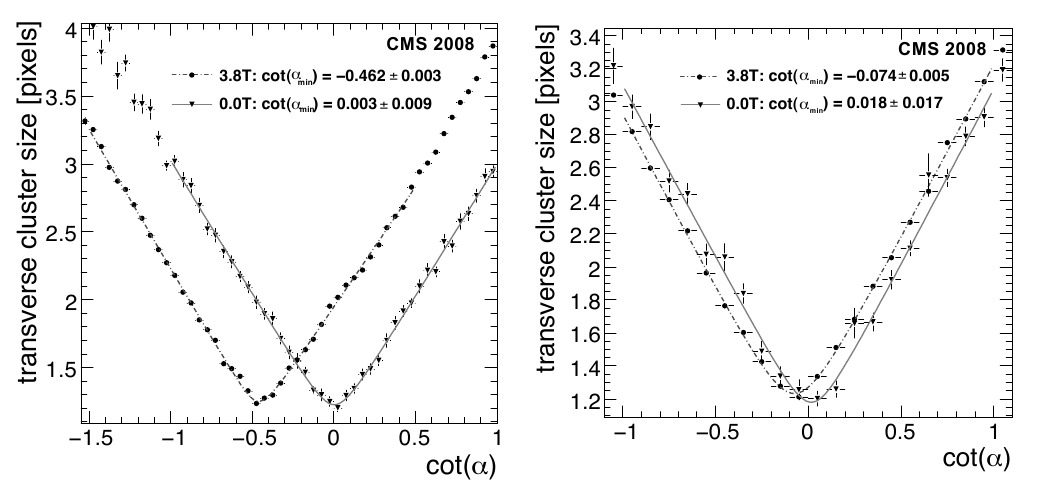
\includegraphics[width=0.6\linewidth]{pixel_clusters.png}
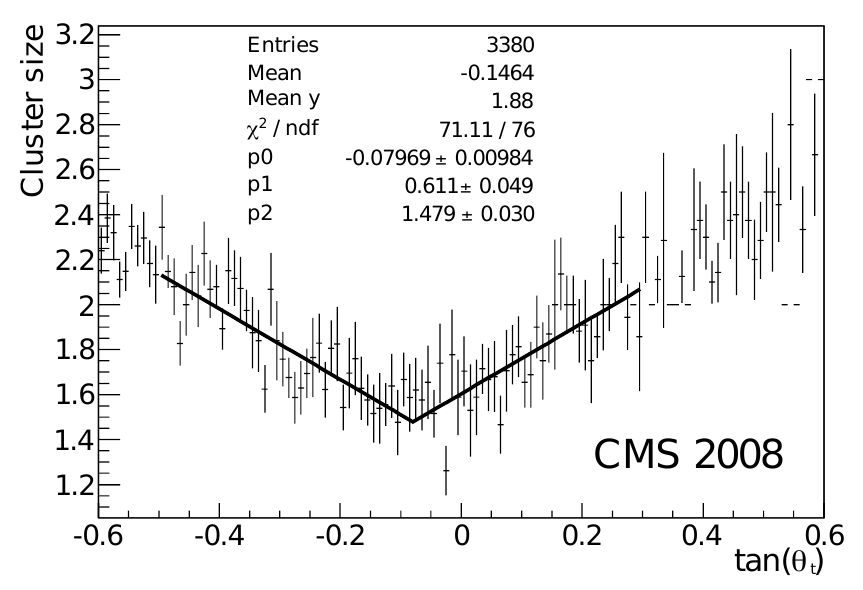
\includegraphics[width=0.4\linewidth]{strip_clusters.png}

\caption{Cluster size versus entrance angle in the pixel barrel
  (left), pixel endcap (middle), with and without magnetic field, and
  TOB layer 4 (right).  High-$p_T$ tracks have minimal entrance
  angle. \label{fig:cluster_size}}
\end{figure}

\begin{figure}[p]
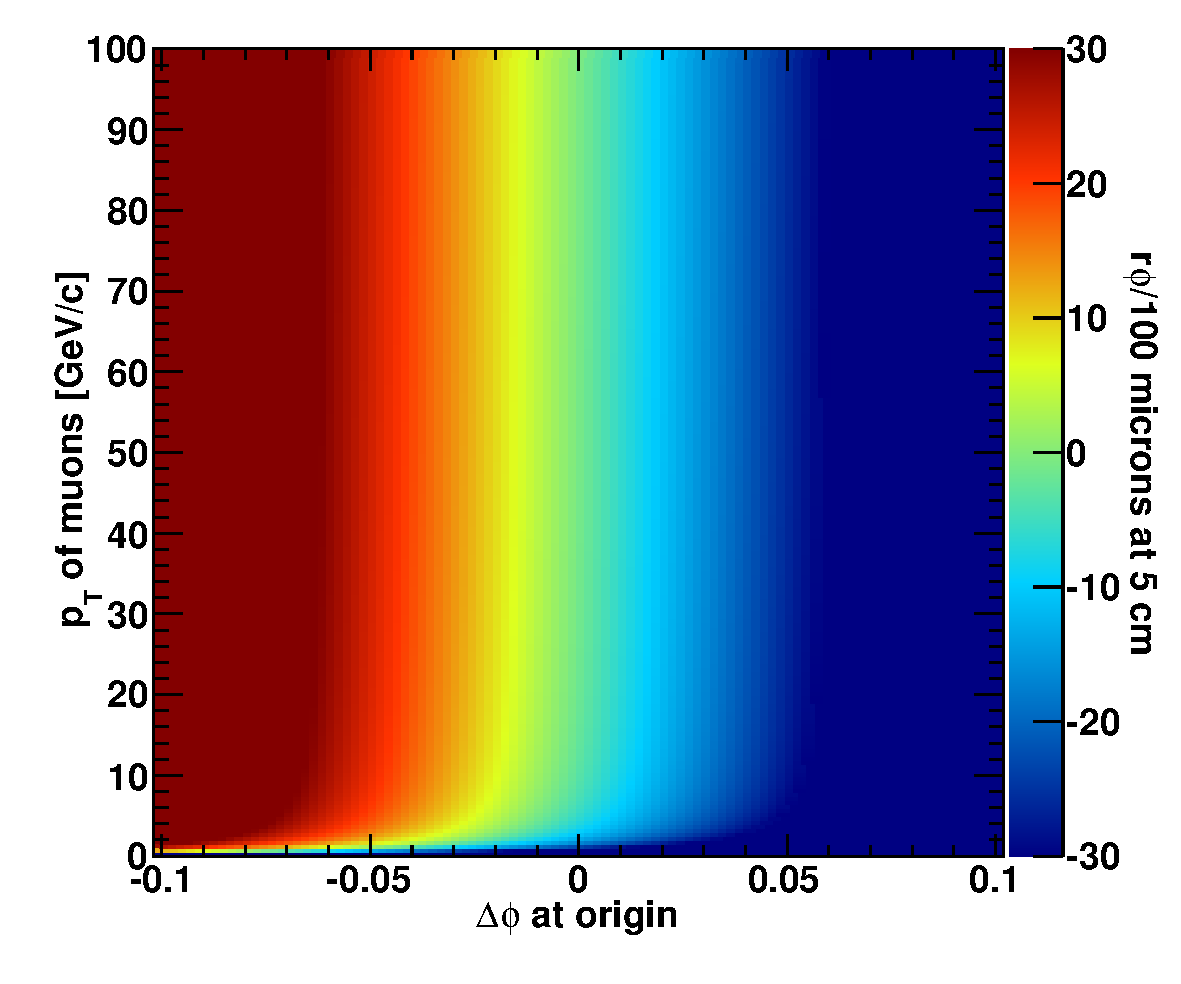
\includegraphics[width=0.5\linewidth]{separation_at_5cm.pdf}
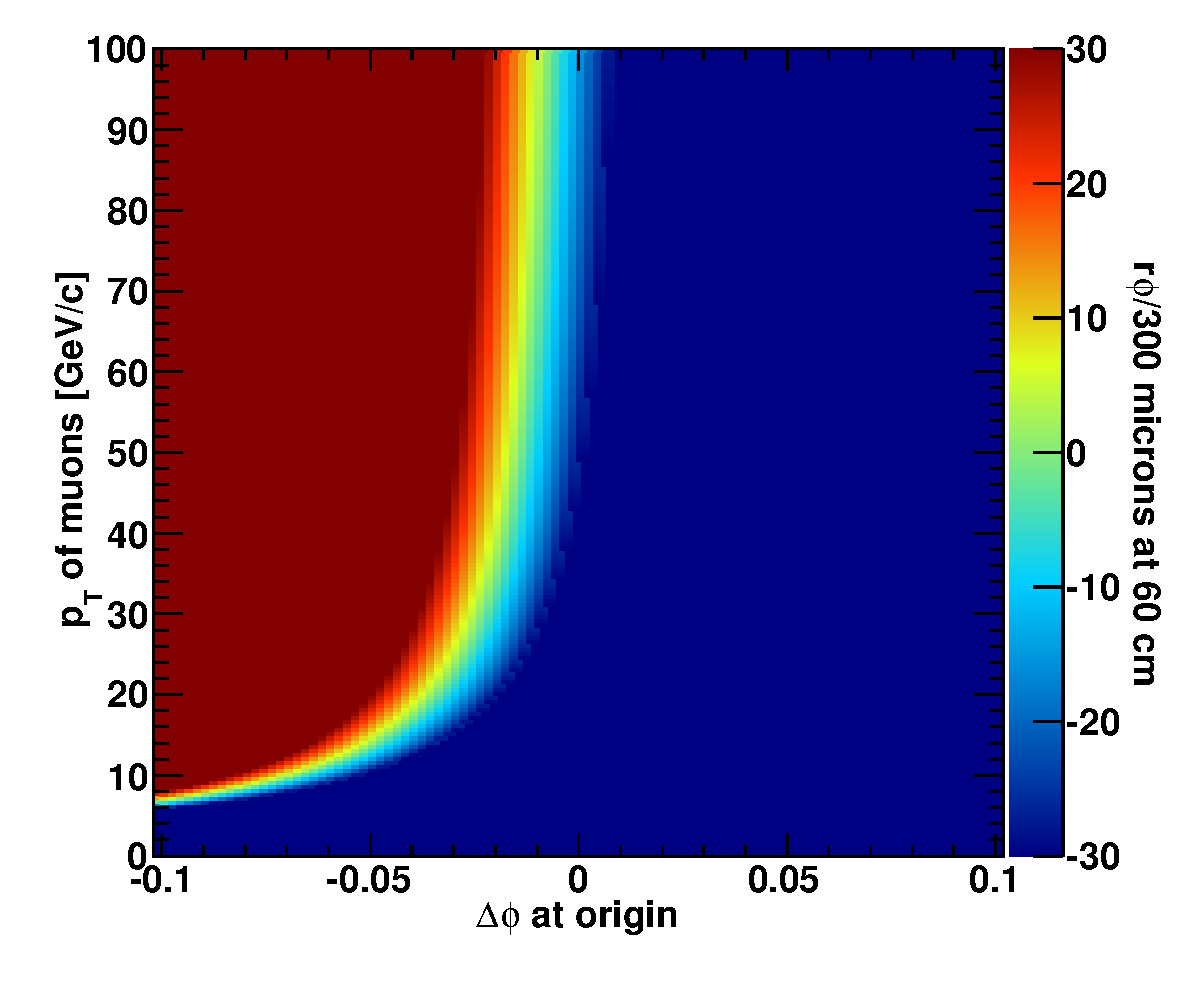
\includegraphics[width=0.5\linewidth]{separation_at_60cm.pdf}

\caption{Separation of two muon trajectories at the first pixel layer,
  5~cm from the beamline (left), and the first TOB layer, 60~cm from
  the beamline (right).  The color scale is the $r\phi$ distance
  between the muon trajectories on a cylinder of the given radius,
  measured in units of channel widths, taking 100~$\mu$m for the pixel
  and 300~$\mu$m for the TOB.  Green is zero separation; red and blue
  are 30 channels apart.  The $r\phi$ separation asymptotically
  approaches a constant multiple of $\Delta \phi$ at the origin for
  high-$p_T$ muons (both muons have the same
  $p_T$ in this simulation). \label{fig:separation}}
\end{figure}

\begin{figure}[p]
\begin{center}
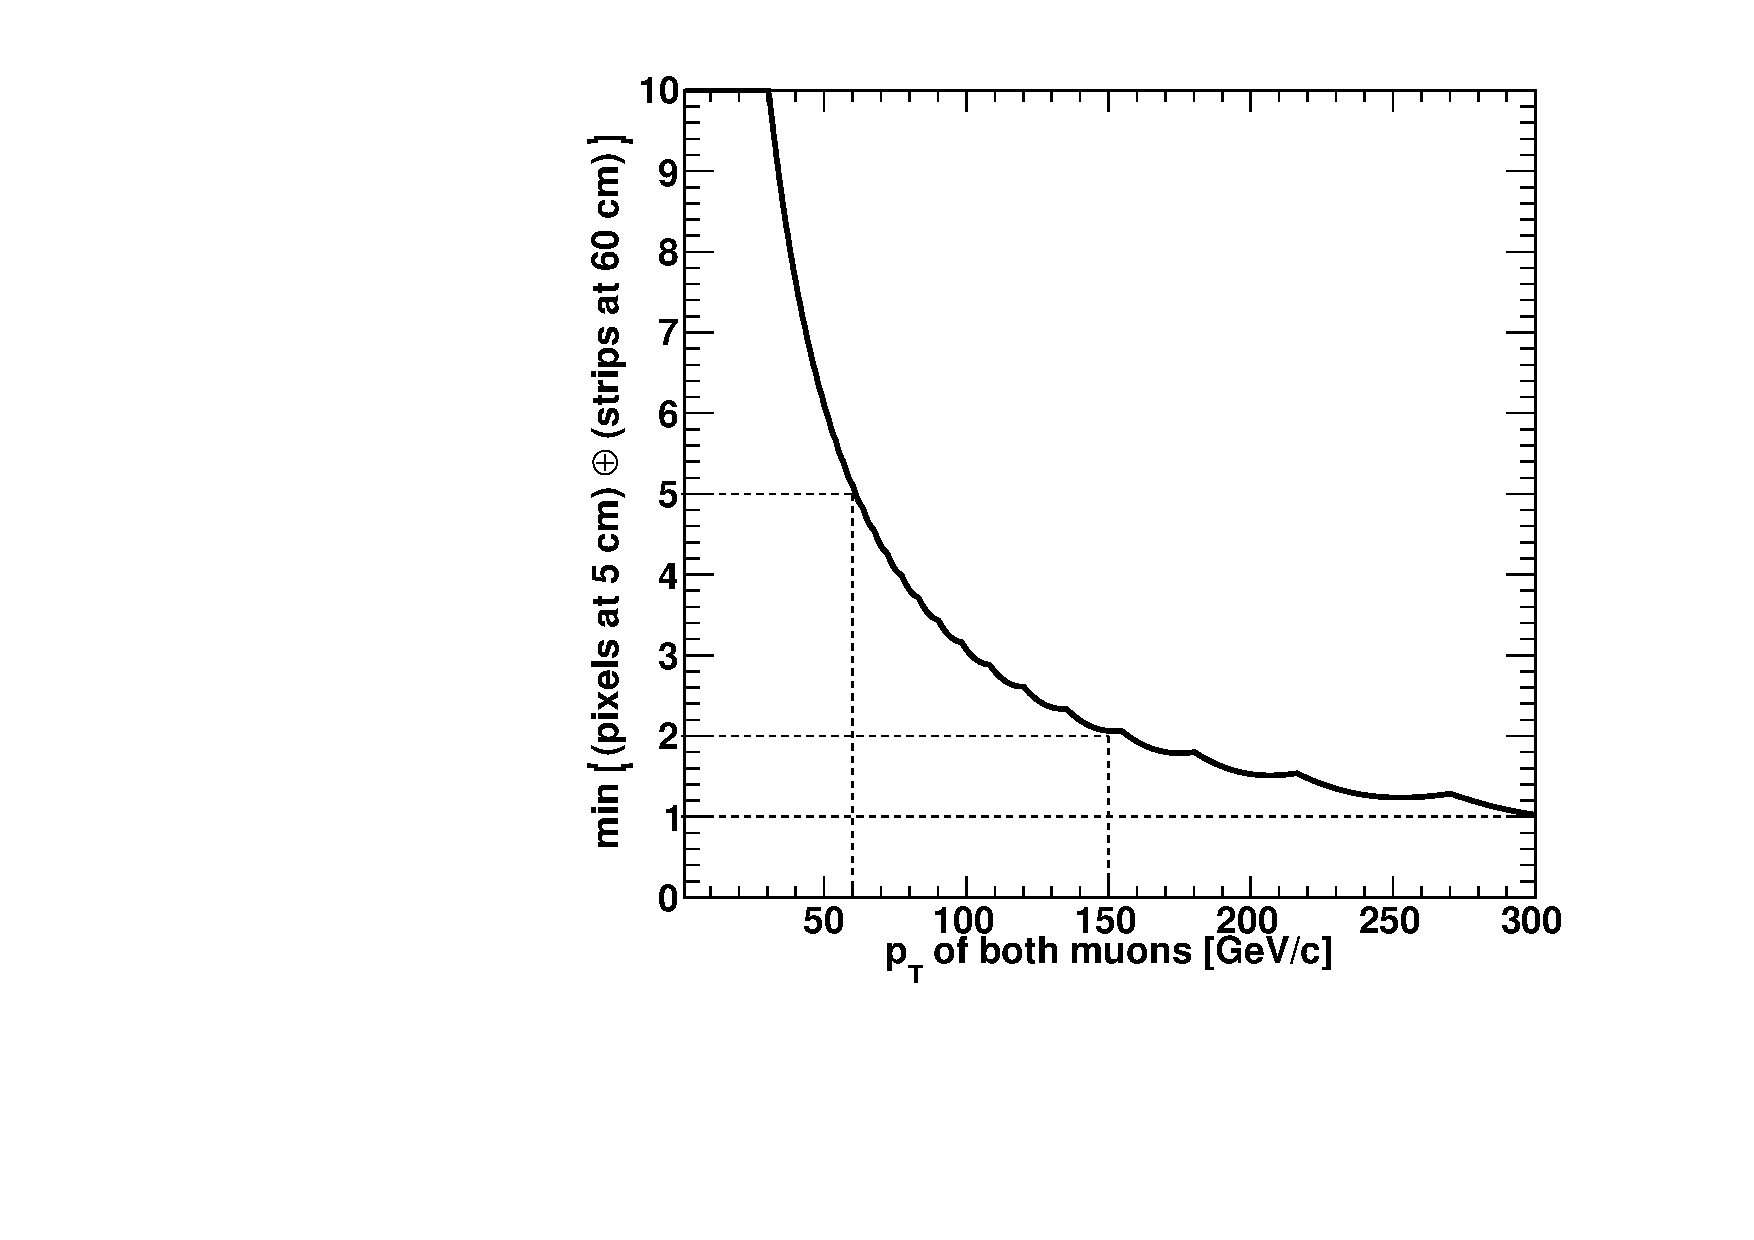
\includegraphics[width=0.5\linewidth]{separation_minimum.pdf}
\end{center}

\caption{Minimum separation in {\it both} the pixel detector at a
  radius of 5~cm {\it and} the TOB at a radius of 60~cm.  The vertical axis
  is the minimum $r\phi$ separation in pixel channel widths, added in
  quadrature with the minimum $r\phi$ separation in TOB channel
  widths, minimized over possible values of $\Delta \phi$ at the
  origin.  For two muons to be separated by $\sim$1 channel width in
  the pixel {\it and} TOB, both muons would need about $p_T \approx
  300$~GeV/$c$. \label{fig:separation2}}
\end{figure}

Figures~\ref{fig:separation} and \ref{fig:separation2} quantify the
degree of separation at two distances from the beamline: 5~cm (first
pixel layer) and 60~cm (first TOB layer, about 50\% through the
tracker).  Two trajectories were propagated from the origin to 5 and
60~cm cylinders using the appropriate CMSSW propagator for a variety
of $\Delta \phi$ opening angles at the origin and initial $p_T$ of
both trajectories (both momenta were equal, with $\eta = 0$).  For a
$\sim$5~channel width separation at both radii, both muons would need
$p_T > 60$~GeV/$c$, for $\sim$2 channel widths, both muons would need
$p_T > 150$~GeV/$c$, and for $\sim$1 channel width, both muons would
need $p_T > 300$~GeV/$c$.

\section{Observing track interference in pair-gun MC}

To search for the onset of an inefficiency due to nearby tracks in the
tracker, I plotted efficiency versus $\Delta R$ using our pair-gun MC.
The pair-gun MC is a full CMSSW simulation of two opposite-sign muons
with uniformly random pair momentum ($0 < p_T^{\mu\mu} <
100$~GeV/$c$), mass ($2m_\mu < m < 6$~GeV/$c^2$), pseudorapidity
($-2.5 < \eta^{\mu\mu} < 2.5$), and azimuthal angle ($-\pi <
\phi^{\mu\mu} < \pi$).  Each pair of muons is reconstructed three
times: once with the $\mu^+$ as the only particle in the event, once
with the $\mu^-$ as the only particle in the event, and once with both
$\mu^+$ and $\mu^-$ in the same event.  This allows us to study
efficiency losses due to interference separately from single-particle
efficiency.

With these tools, we can define ``interference efficiency'' in the
following way:
\begin{equation}
P(\mu^+\mu^- | \mu^+\mbox{ and }\mu^-) = \frac{\mbox{both muons
  reconstructed in the same event and separately}}{\mbox{both muons
    reconstructed separately}}
\end{equation}
with additional generator-level requirements of $p_T > 5$~GeV/$c$
and $|\eta| < 2.4$ for both numerator and denominator.
``Reconstructed'' means that the reconstructed track exists with $\ge
8$ hits and $\chi^2/N_\s{dof} < 4$, though these quality cuts have
negligible impact on the final result.  The probability of
reconstructing both muons separately, given kinematical acceptance, is
99.6\%.

Figure~\ref{fig:doubleeff} presents this interference efficiency as a
function of $\Delta R$, where an 8\% dip is visible for $\Delta R <
0.01$.  This dip is correlated with high momentum (same figure),
suggesting that it is related to track overlap.  For context, we show
the mass distribution of muon pairs with $\Delta R < 0.01$ in this
sample in Fig.~\ref{fig:doubleeff_mass}.  The 100~GeV/$c$ upper limit
in momentum implies only mass $<$ 0.5~GeV/$c^2$ pairs have such a
small opening angle.  For a 1~GeV/$c^2$ boson, the onset of the effect
would be at higher momenta.

\begin{figure}
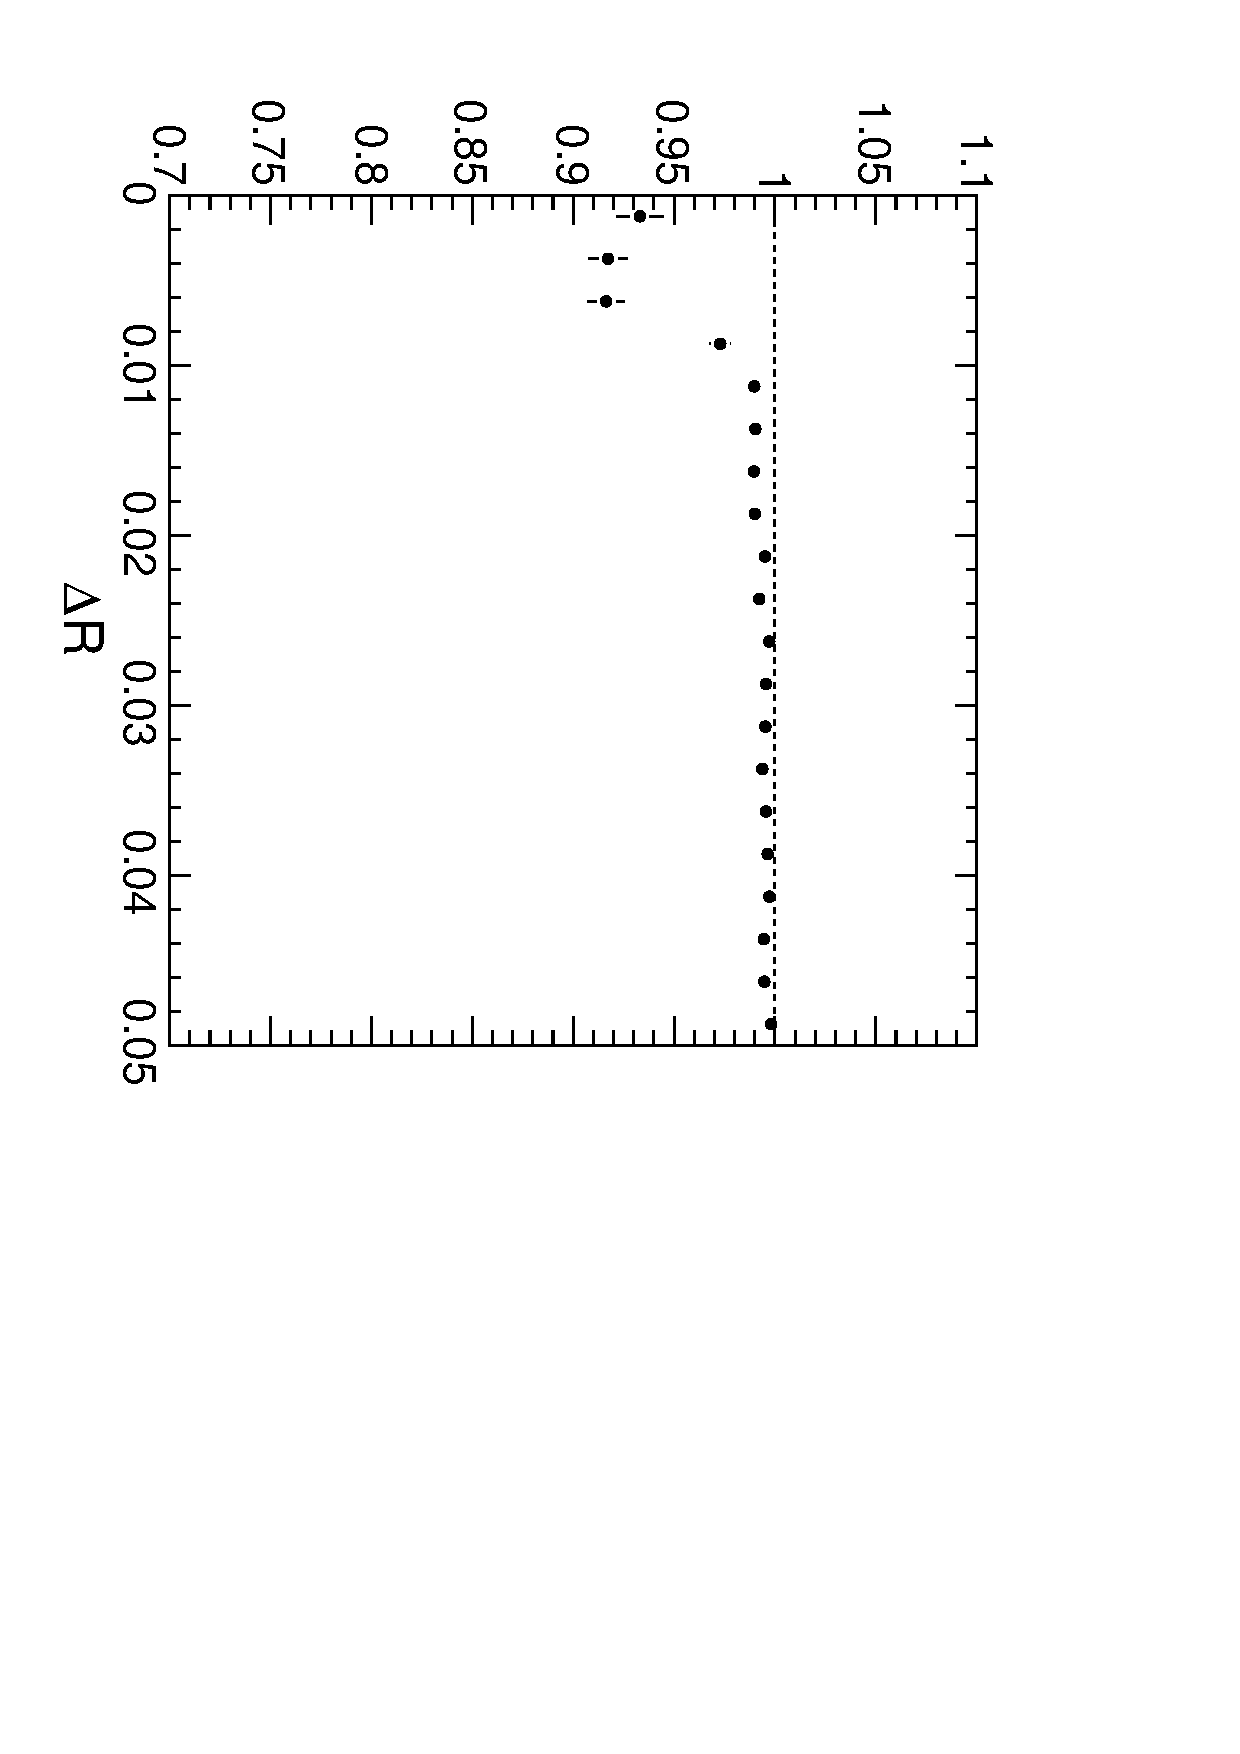
\includegraphics[height=0.5\linewidth, angle=90]{doubleeff_deltar.pdf}
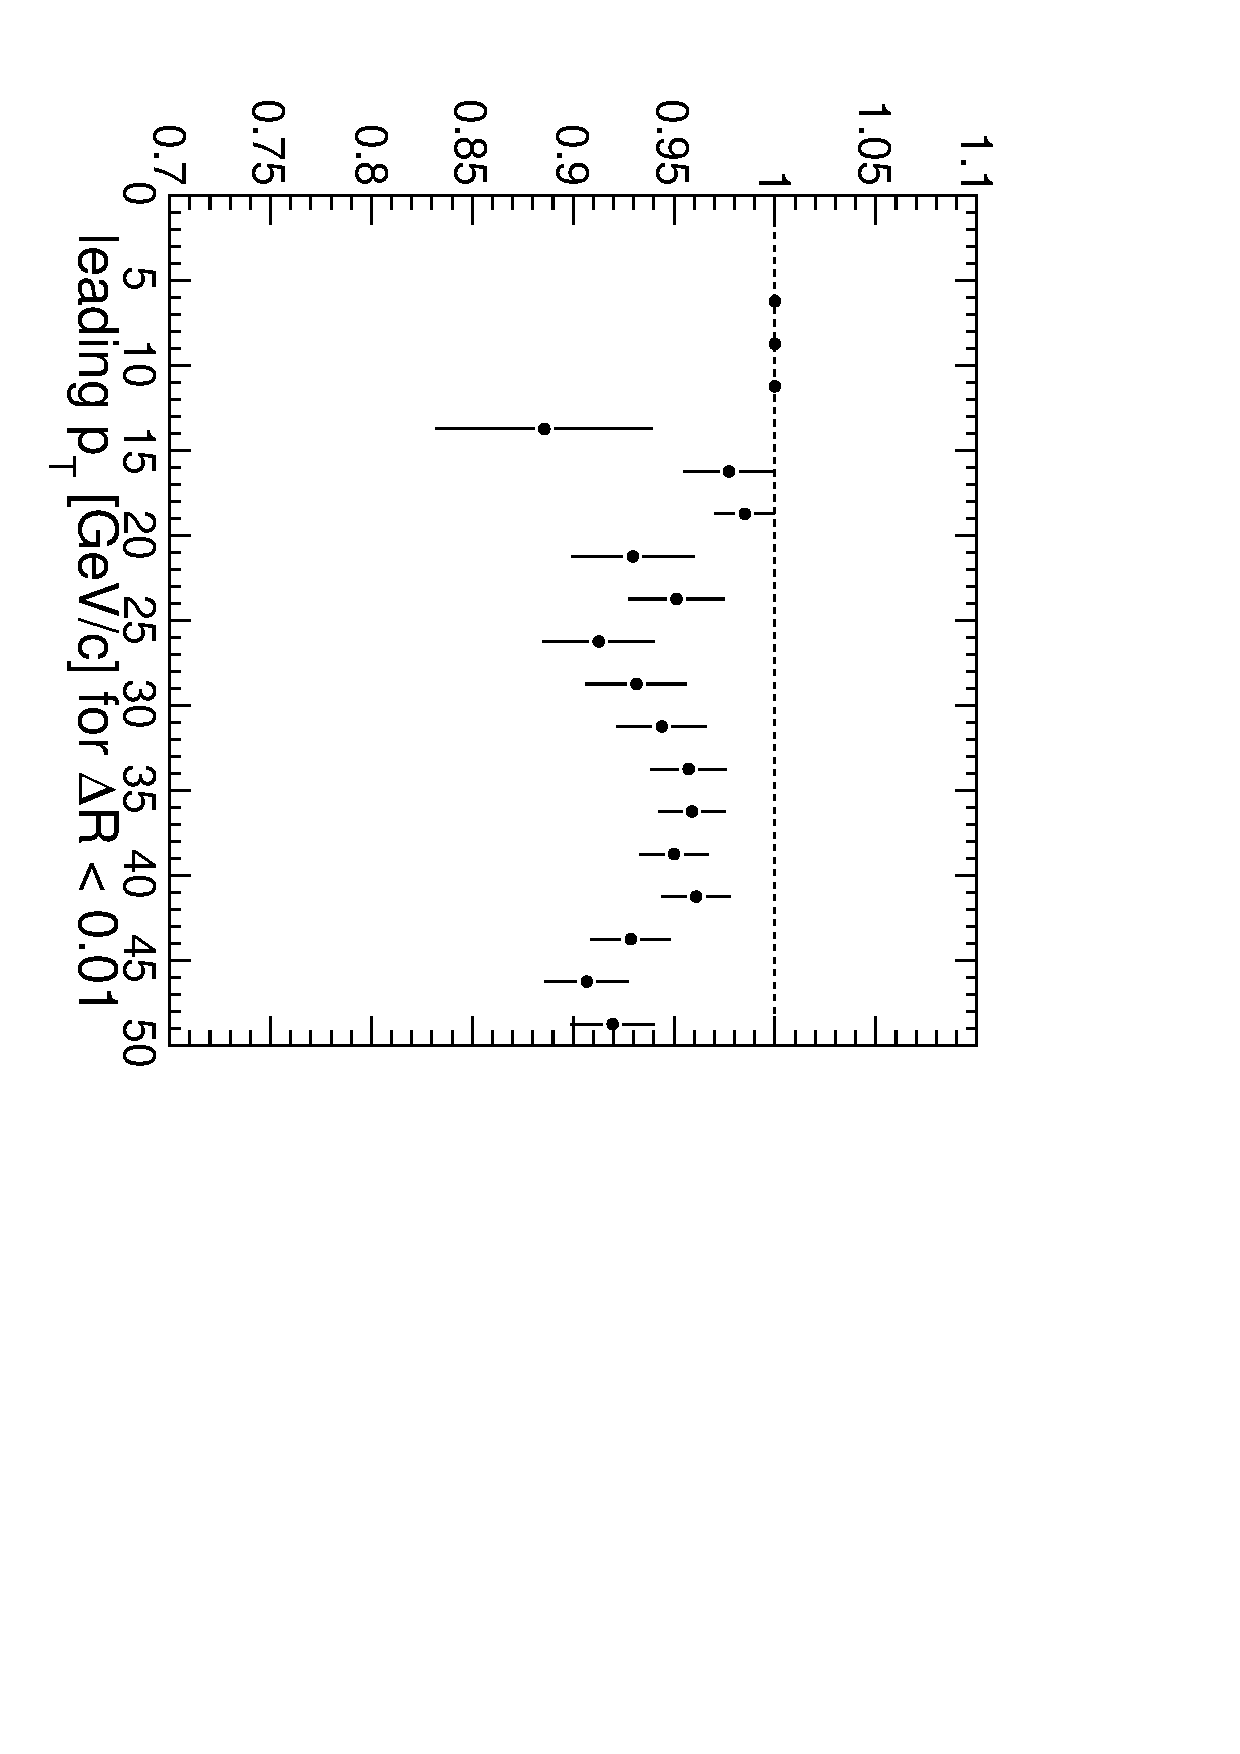
\includegraphics[height=0.5\linewidth, angle=90]{doubleeff_leadpt.pdf}

\caption{Left: $P(\mu^+\mu^- | \mu^+\mbox{ and }\mu^-)$ for track cuts
  (see text) versus $\Delta R$.  Right: the same quantity versus
  leading muon $p_T$ for $\Delta R < 0.01$, showing that the effect
  prefers high momenta. \label{fig:doubleeff}}
\end{figure}

\begin{figure}
\begin{center}
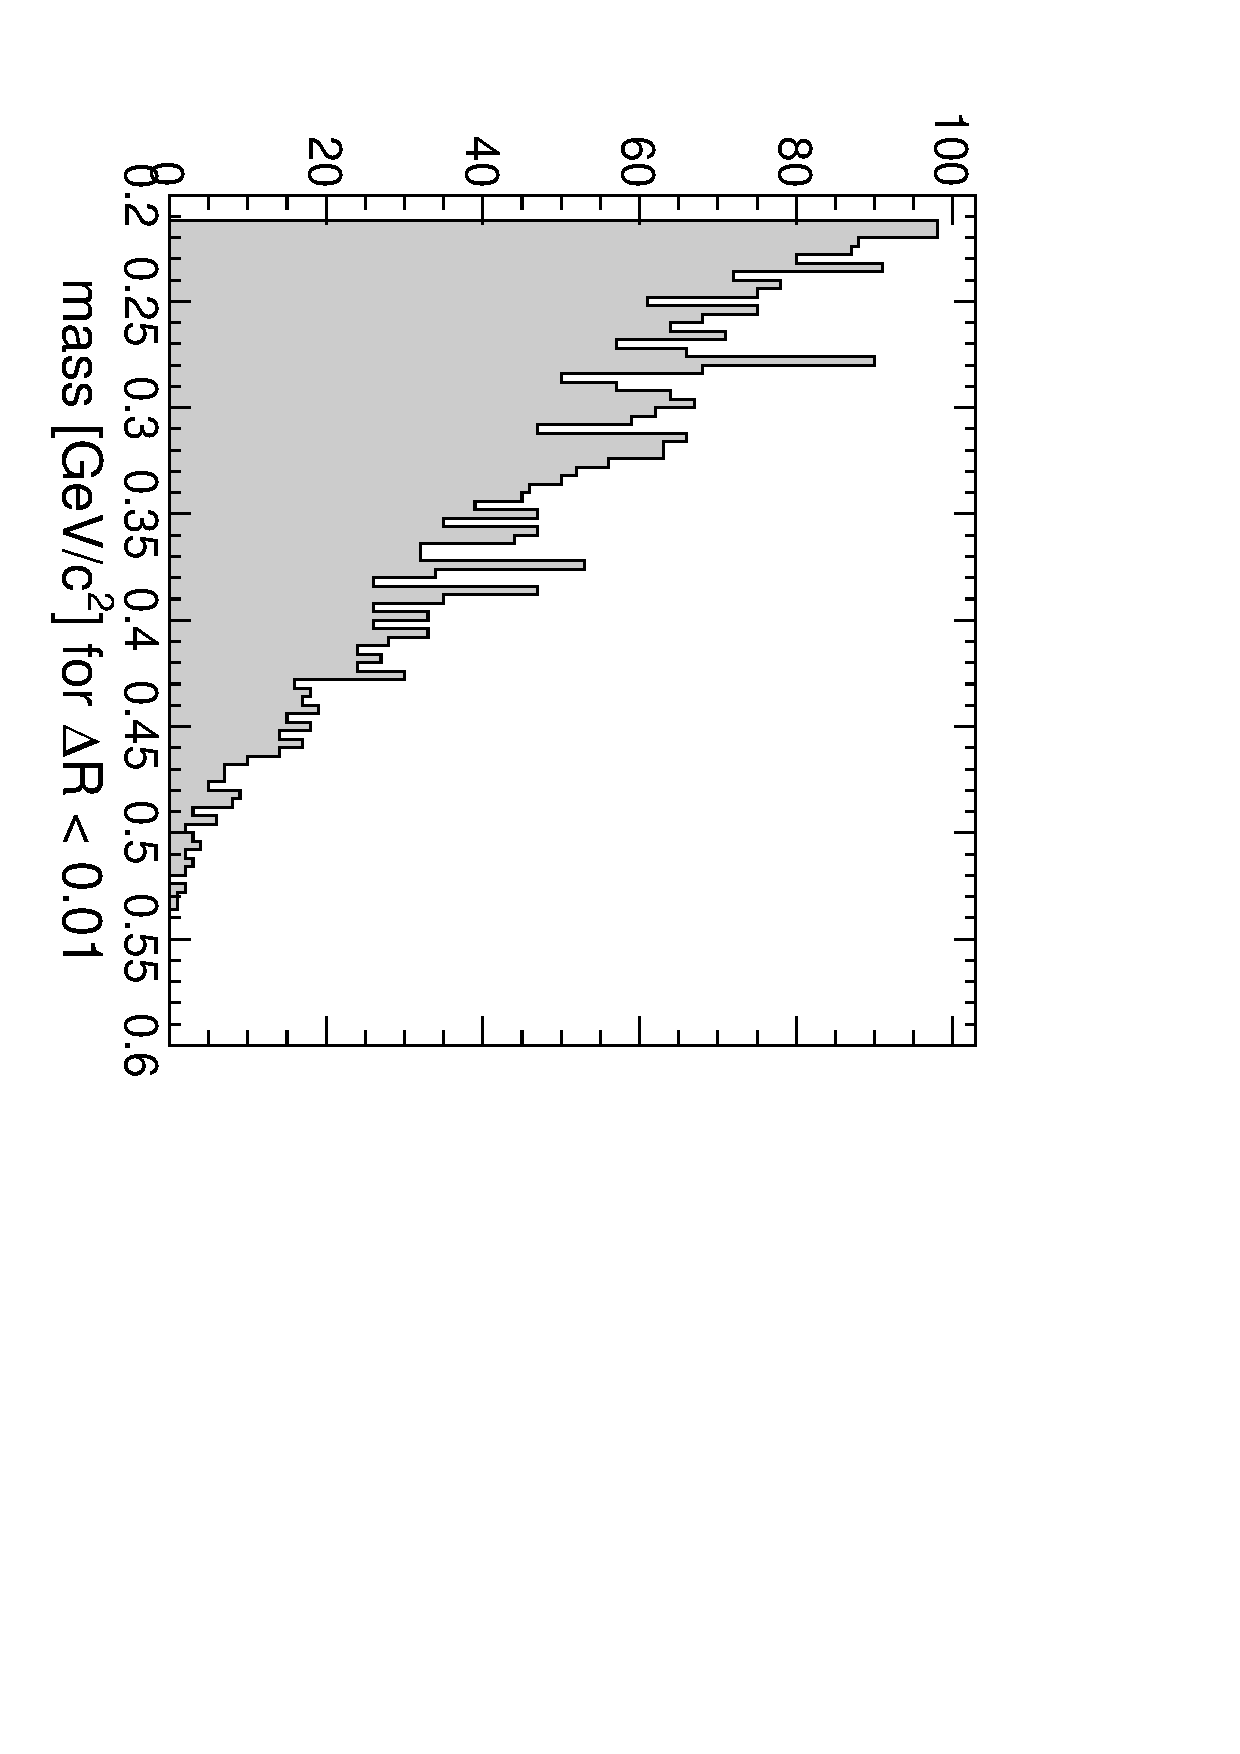
\includegraphics[height=0.5\linewidth, angle=90]{doubleeff_mass.pdf}
\end{center}

\caption{Values of muon pair mass consistent with $\Delta R < 0.01$ in
  this simulation, for context. \label{fig:doubleeff_mass}}
\end{figure}

The same study can be performed for the full muon cuts, that is,
adding the requirement that the track is reconstructed as a
TrackerMuon with $\ge 2$ arbitrated muon segments.  This is presented
in Fig.~\ref{fig:doubleeff_muon}.  The interference efficiency for the
full muon cuts has the same shape as a function of $\Delta R$, though
a lower plateau for $\Delta R \gg 0.01$.  This is the effect of
the muons crossing the muon system (discussed in the analysis note),
which is not a strict fuction of $\Delta R$ at the origin.

\begin{figure}
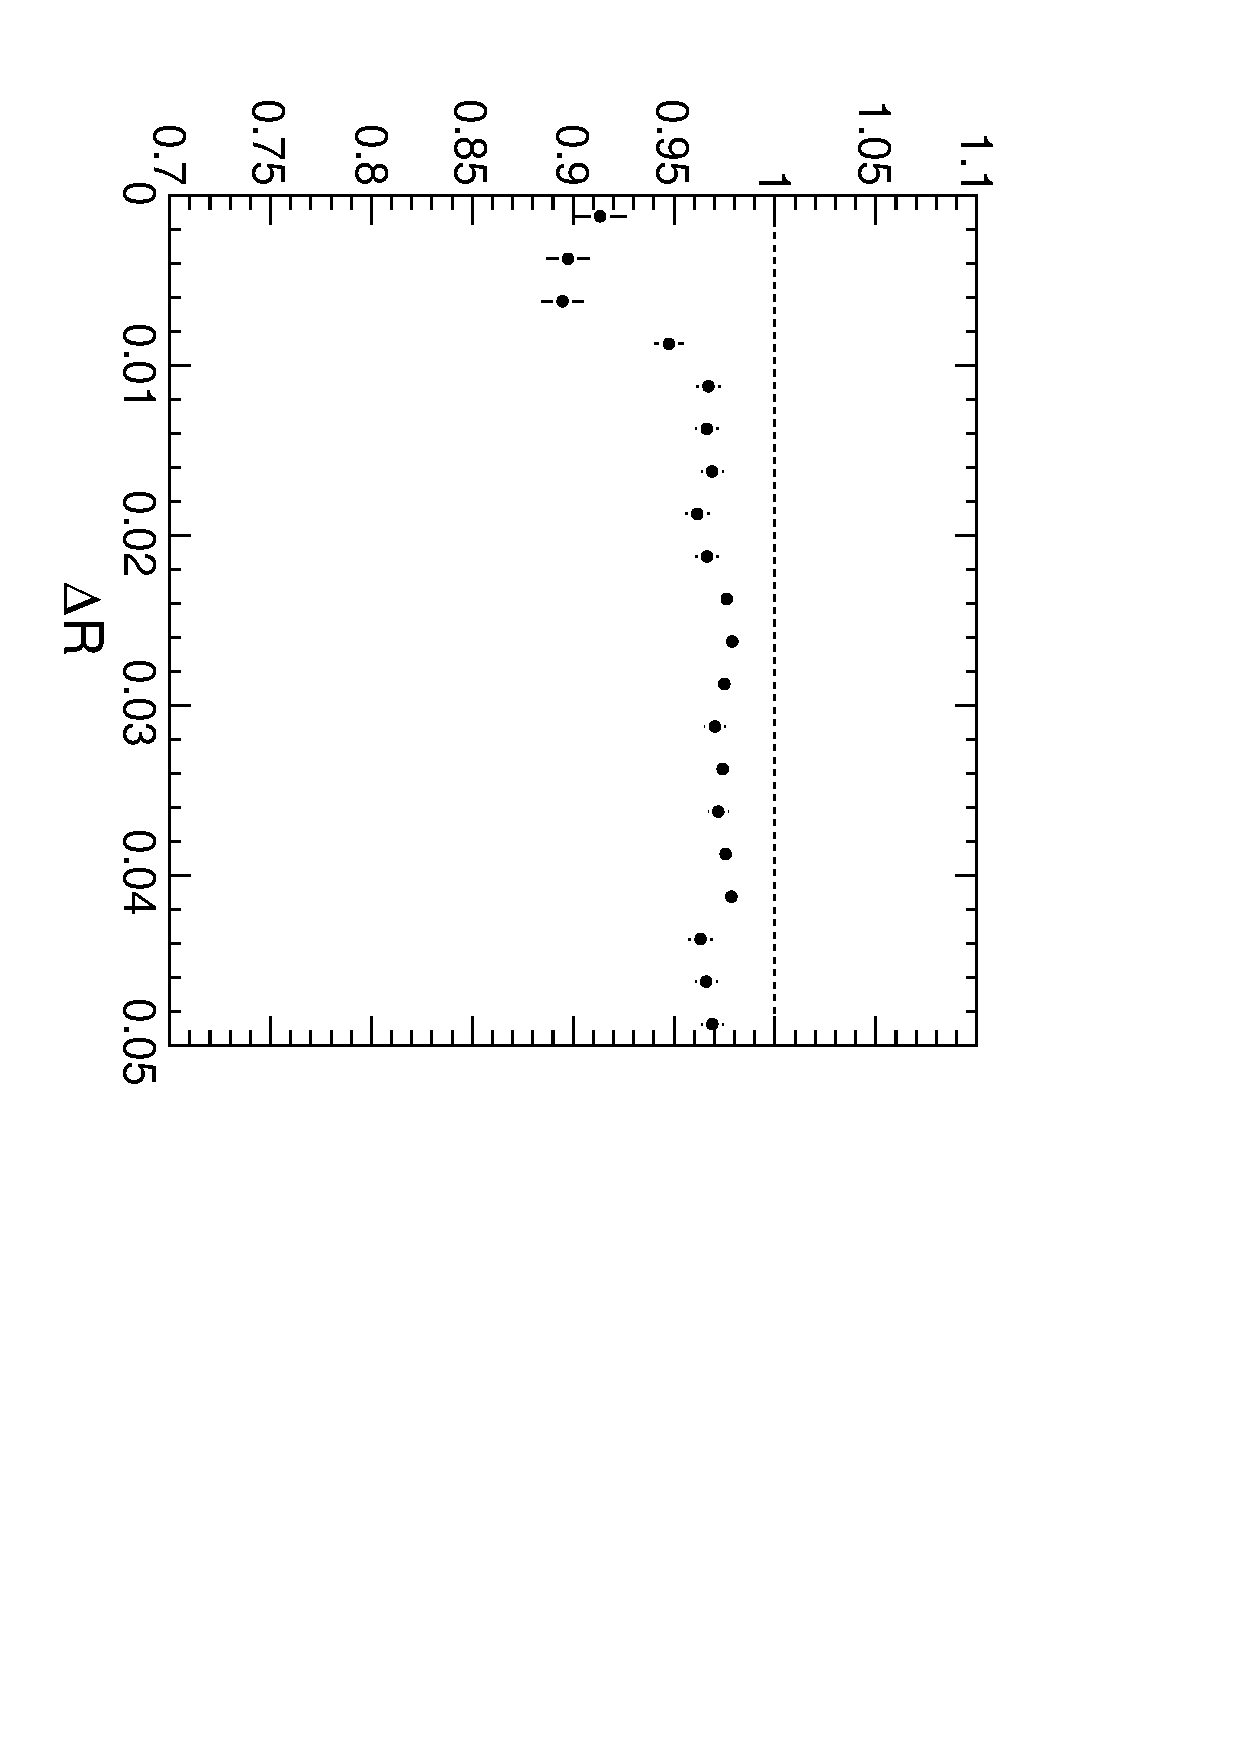
\includegraphics[height=0.5\linewidth, angle=90]{doubleeff_deltar_muon.pdf}
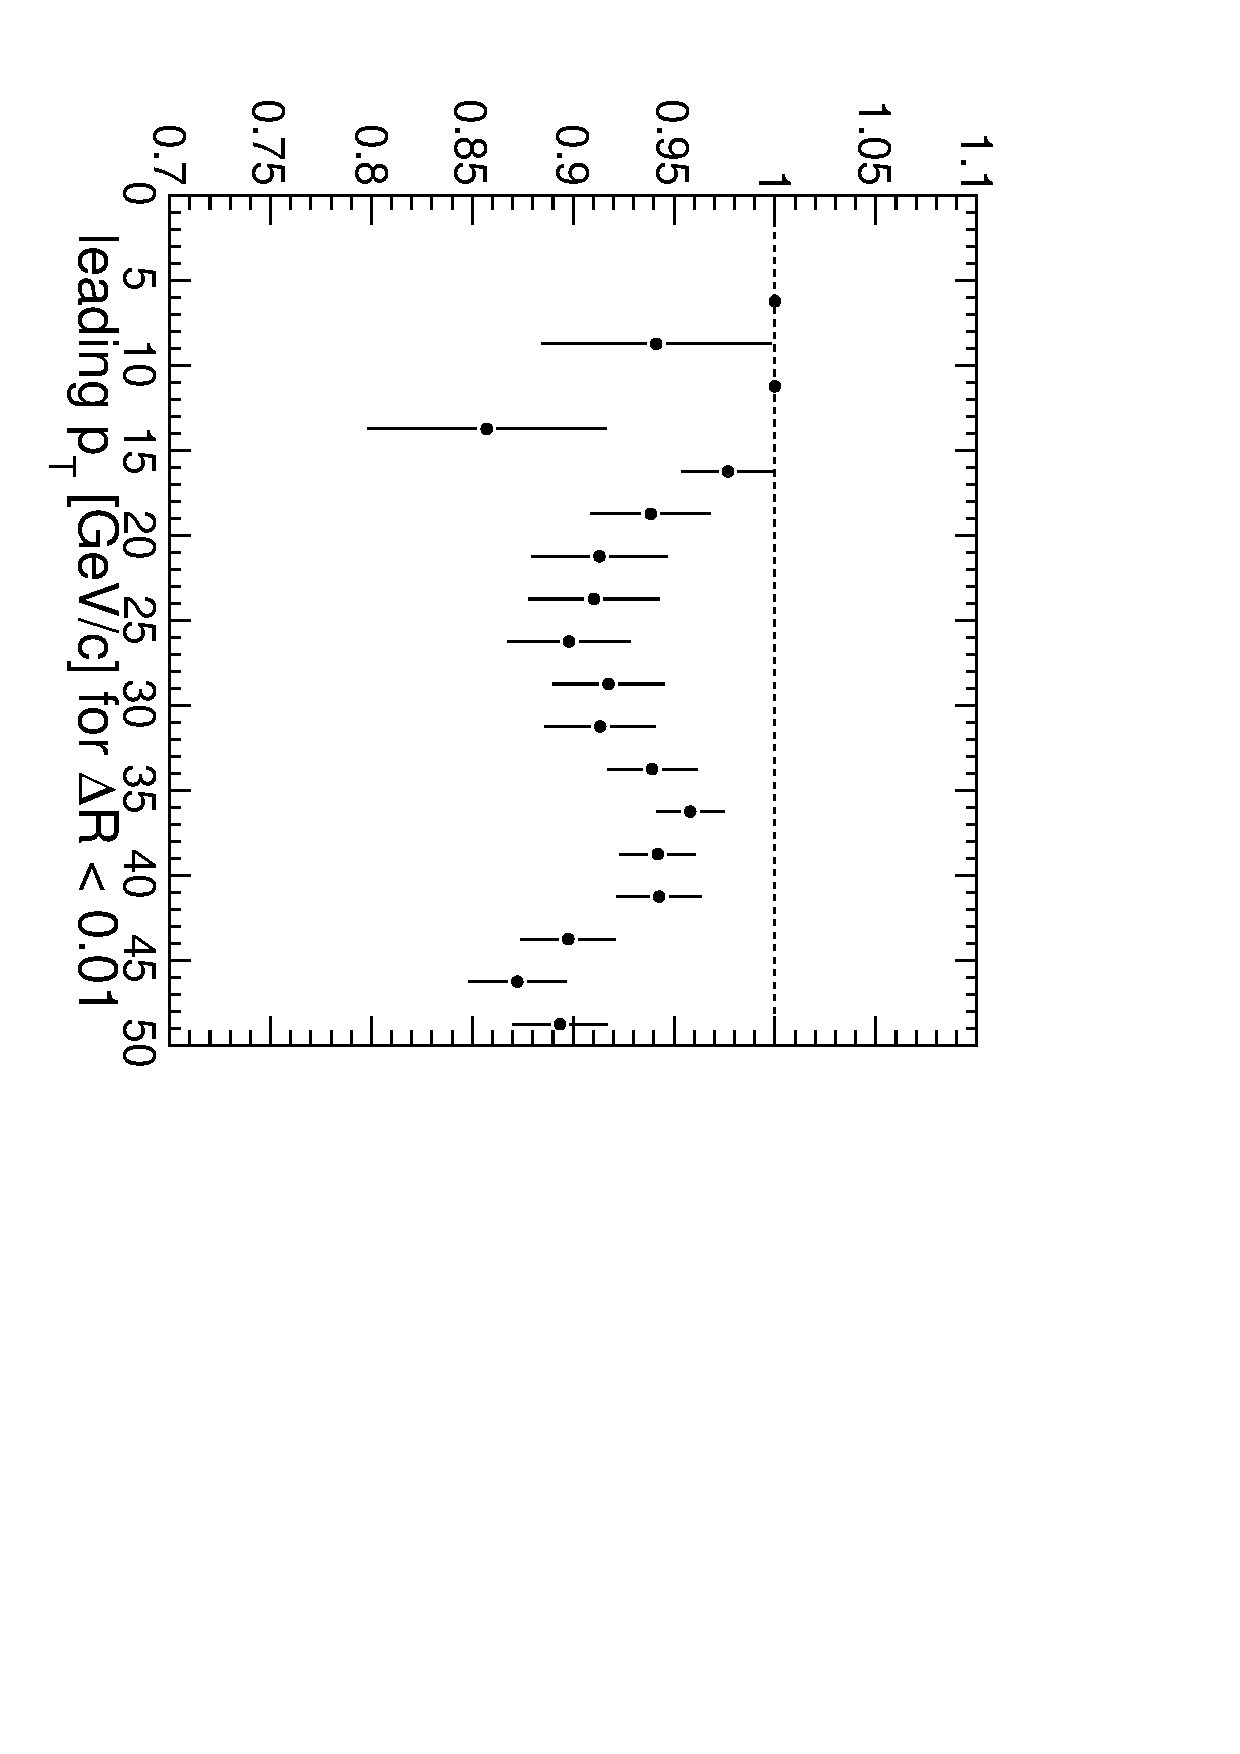
\includegraphics[height=0.5\linewidth, angle=90]{doubleeff_leadpt_muon.pdf}

\caption{Left: $P(\mu^+\mu^- | \mu^+\mbox{ and }\mu^-)$ for muon cuts
  versus $\Delta R$.  Right: the same quantity versus leading muon
  $p_T$ for $\Delta R < 0.01$, showing that the effect prefers high
  momenta. \label{fig:doubleeff_muon}}
\end{figure}

\section{Data/MC comparisons for tracking}

The {\it CMS Tracking Performance Results from early LHC Operation}
paper (\url{http://arxiv.org/abs/1007.1988}) presents a detailed
overview of the status of the tracking simulation with early
collisions.  The simulation is shown to reproduce the shapes of signal
responses (see Fig.~\ref{fig:cluster_charge}, copied from the paper)
and many high-level tracking quantities.  Figure~\ref{fig:ourcuts}
shows the number of hits and $\chi^2/N_\s{dof}$ distributions from
this paper, which are relevant to our analysis as track quality cuts.
The distributions in the early LHC paper represent low-$p_T$ hadrons,
rather than $p_T > 5$~GeV/$c$ muons, though.

\begin{figure}
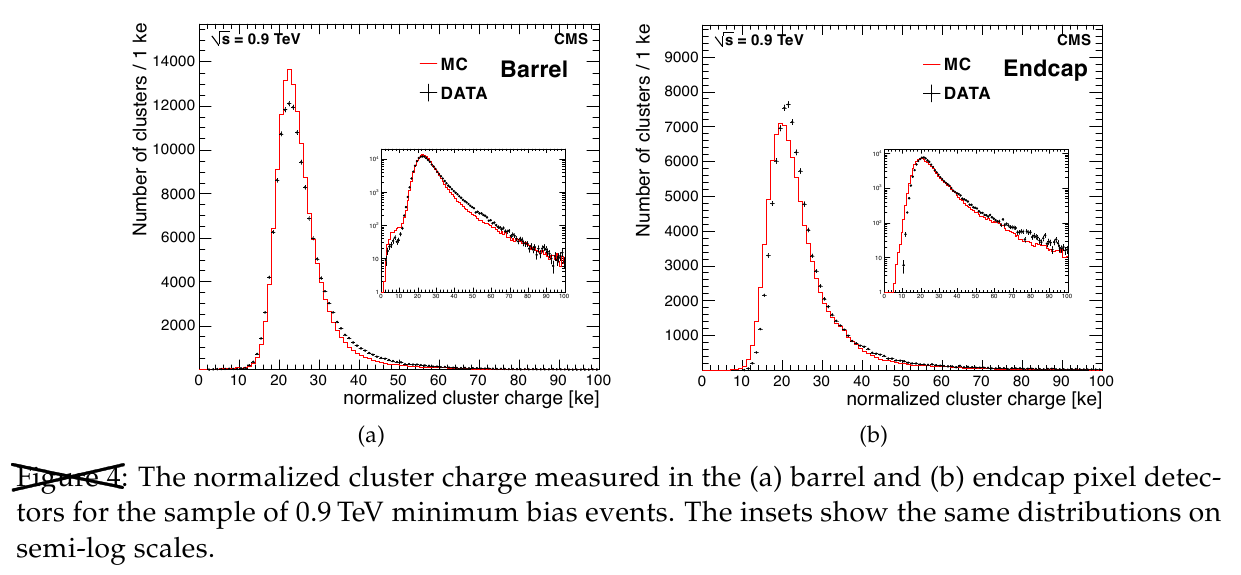
\includegraphics[width=\linewidth]{cluster_charge.png}

\caption{Figure reproduced from the early LHC tracking
  paper. \label{fig:cluster_charge}}
\end{figure}

\begin{figure}
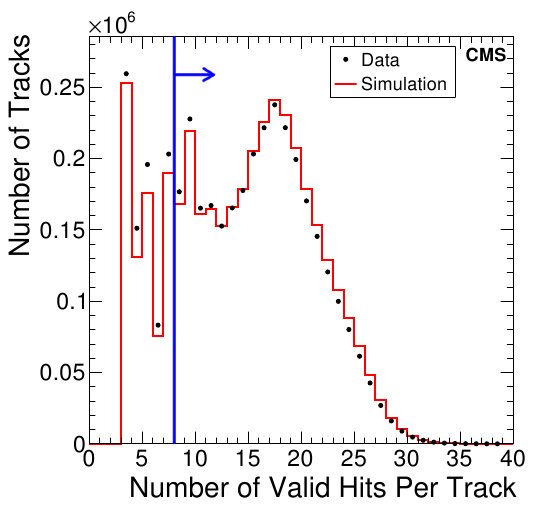
\includegraphics[width=0.5\linewidth]{number_of_hits.png}
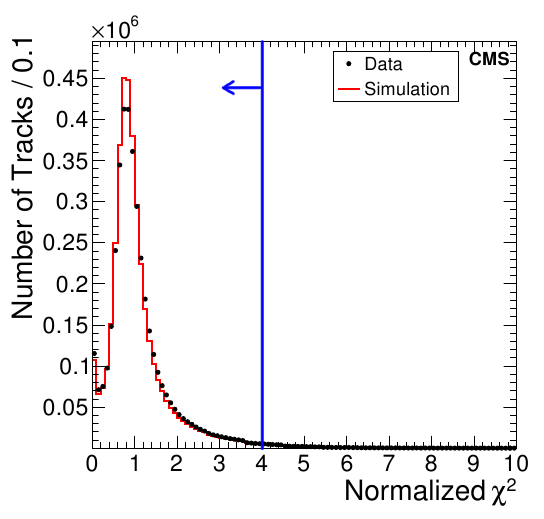
\includegraphics[width=0.5\linewidth]{normalized_chi2.png}

\caption{Two figures from the early LHC tracking paper relevant to our
  analysis: blue lines indicate our cuts.  These distributions have
  different shapes for our $p_T > 5$~GeV/$c$
  tracks. \label{fig:ourcuts}}
\end{figure}

One may argue that the tracking simulation may be trusted if it
reproduces all low-level signals and has a realistic alignment, since
our analysis signal only differs in geometry, and all geometry and
algorithms are the same for data and Monte Carlo.  This can be
partially tested with studies of the $\phi(1020)$ resonance.

\section{Study of the $\phi(1020)$ resonance}

The $\phi(1020)$ resonance provides a standard candle of low-mass,
moderately high-momentum dimuons with which to test the level of
data/MC agreement.  It corresponds to a moderately low range of
opening angles $0.05 < \Delta R < 0.15$, though not low enough to
sample the $\Delta R < 0.01$ tracker inefficiency.  It is the
lowest-mass Standard Model narrow resonance found in both data and
Monte Carlo ($\omega(782) \to \mu\mu$ is missing from the Pythia~6
decay tables), and it is in the middle of the target mass range of our
analysis, though lower than our target momentum range.

Figure~\ref{fig:phi_mass} presents the invariant mass distribution
near the $\phi(1020)$ peak, indicating the signal region ($|m -
m_\phi| < 0.025$~GeV/$c^2$), the sidebands ($0.050 < |m -
m_\phi| < 0.075$~GeV/$c^2$), and a pure $\phi(1020)$ Monte Carlo
simulation.  The $\phi(1020)$ simulation is a subset of
InclusiveMu5\_Pt30 (muons from Pythia 6 QCD): dimuons selected at
generator level to have $\phi(1020)$ as their parent.

\begin{figure}
\begin{center}
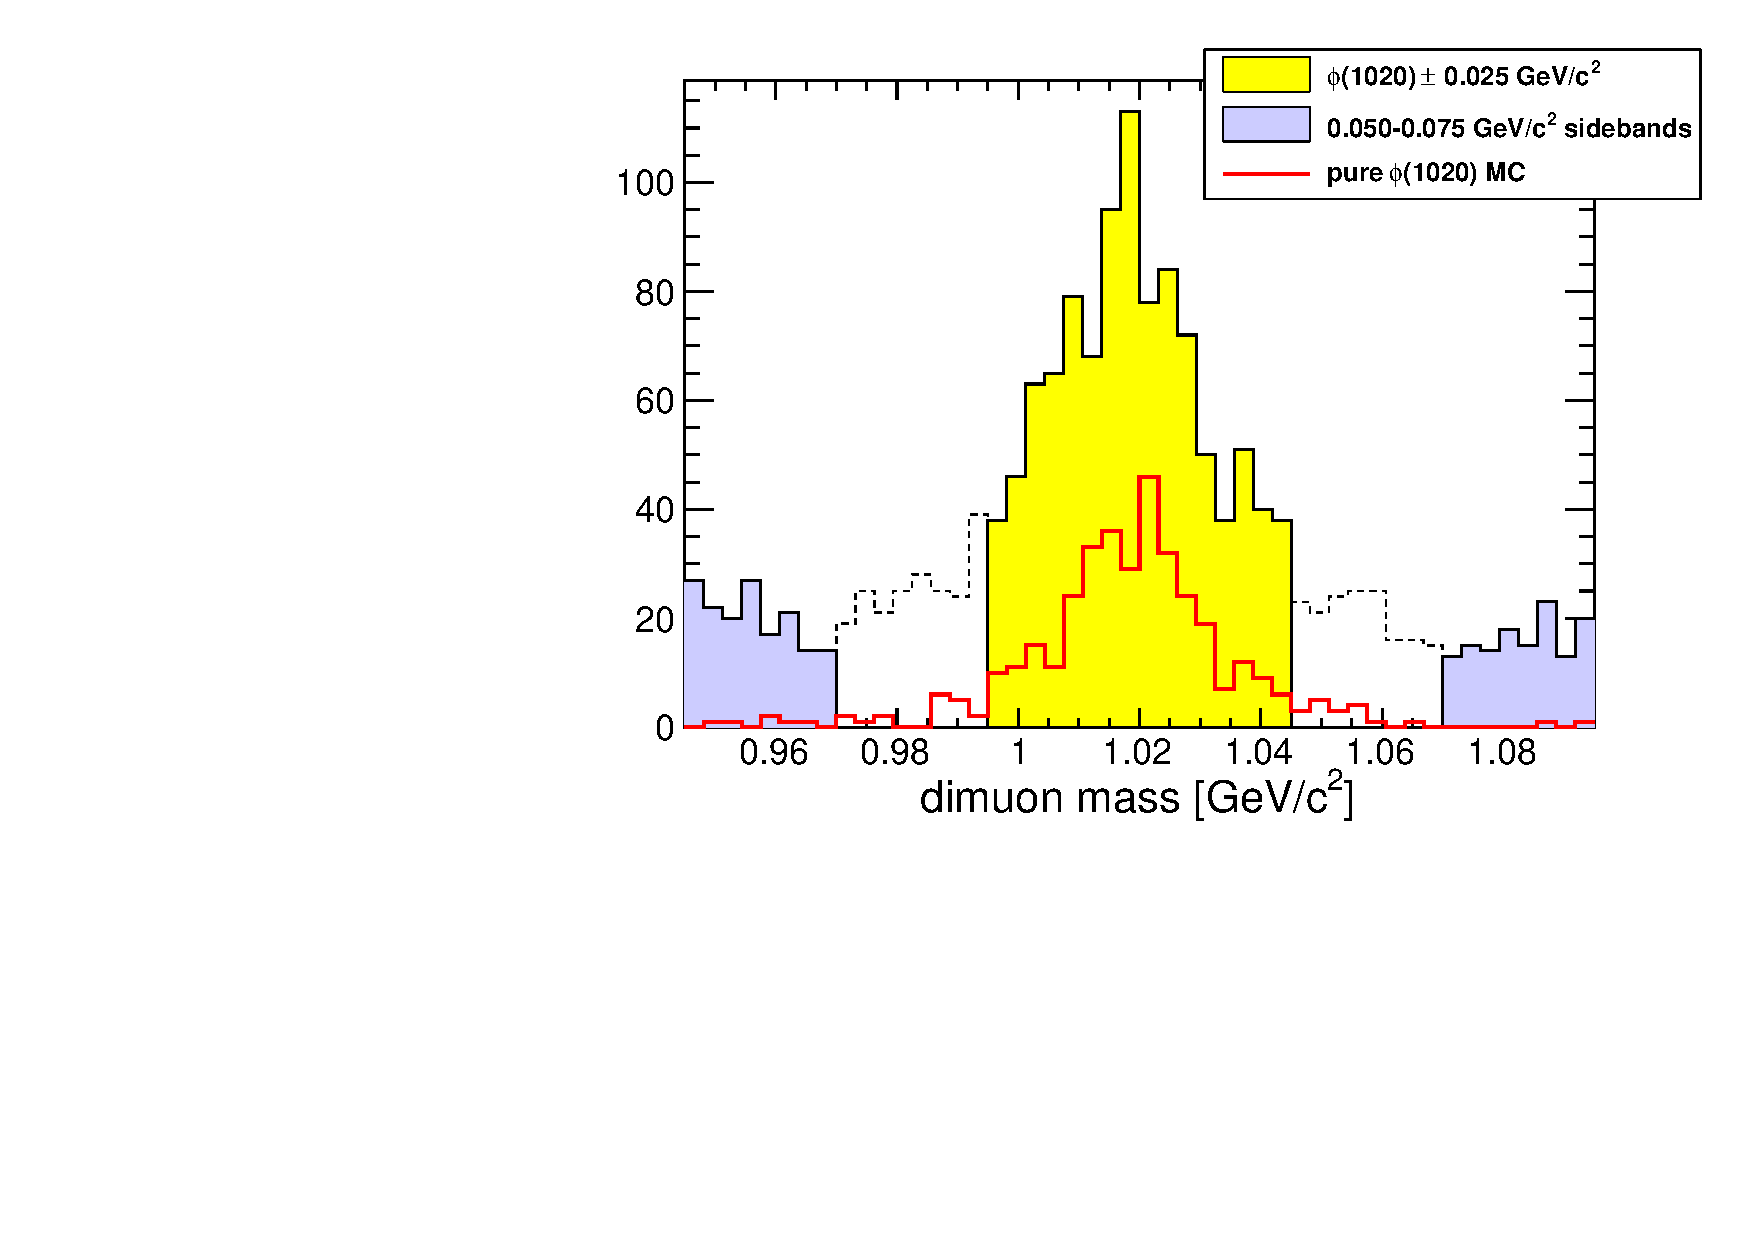
\includegraphics[width=0.75\linewidth]{phi_mass.pdf}
\end{center}

\caption{Basic distribution of the $\phi(1020)$ study: dimuon
  invariant mass distribution of data (dashed line, colored in
  sections) with the signal region indicated by yellow, the sidebands
  indicated by blue, overlaid with a pure $\phi(1020)$ MC simulation
  (unscaled). \label{fig:phi_mass}}
\end{figure}

The $\phi(1020)$ events in Monte Carlo are all prompt and in jets,
while the data has a displaced component and an isolated component.
For a more appropriate comparison, I applied the following cuts:
\begin{itemize}
\item distance between the dimuon vertex and the closest primary
  vertex in $z$ must be less than 1~mm ($L_{xy} < 1$~mm);
\item the sum of track $p_T$ for $p_T > 1.5$~GeV/$c$ in a $\Delta R <
  0.4$ cone around the dimuon axis must be greater than 3~GeV/$c$
  ($Iso > 3$~GeV/$c$);
\item exactly two reconstructed muons per event;
\item apply $|m - m_\phi| < 0.025$~GeV/$c^2$ to Monte Carlo as well as
  the signal;
\item at least one muon must have $p_T > 10$~GeV/$c$.
\end{itemize}
The data were collected using any single or double-muon trigger that
was available.  Prescales changed during the run, but HLT\_Mu9 and
HLT\_Mu11 were prescaled late in the year--- the requirement of $p_T >
10$~GeV/$c$ is a compromise between strict correctness (our analysis
uses only $p_T > 15$~GeV/$c$) and the need to maximize the size of the
dataset for statistically meaningful comparisions.
Figure~\ref{fig:phi_muon12pt} shows sideband-subtracted $\phi(1020)$
data overlaid by normalized Monte Carlo of the highest and
lowest-$p_T$ muon in each event.  The data and Monte Carlo $p_T$
spectra are consistent: there is no evidence of trigger prescale
thresholds in the spectrum.  Figure~\ref{fig:phi_other} presents the
$\Delta R$, $\eta$, $Iso$, and $L_{xy}$ distributions (with all cuts
applied).

\begin{figure}
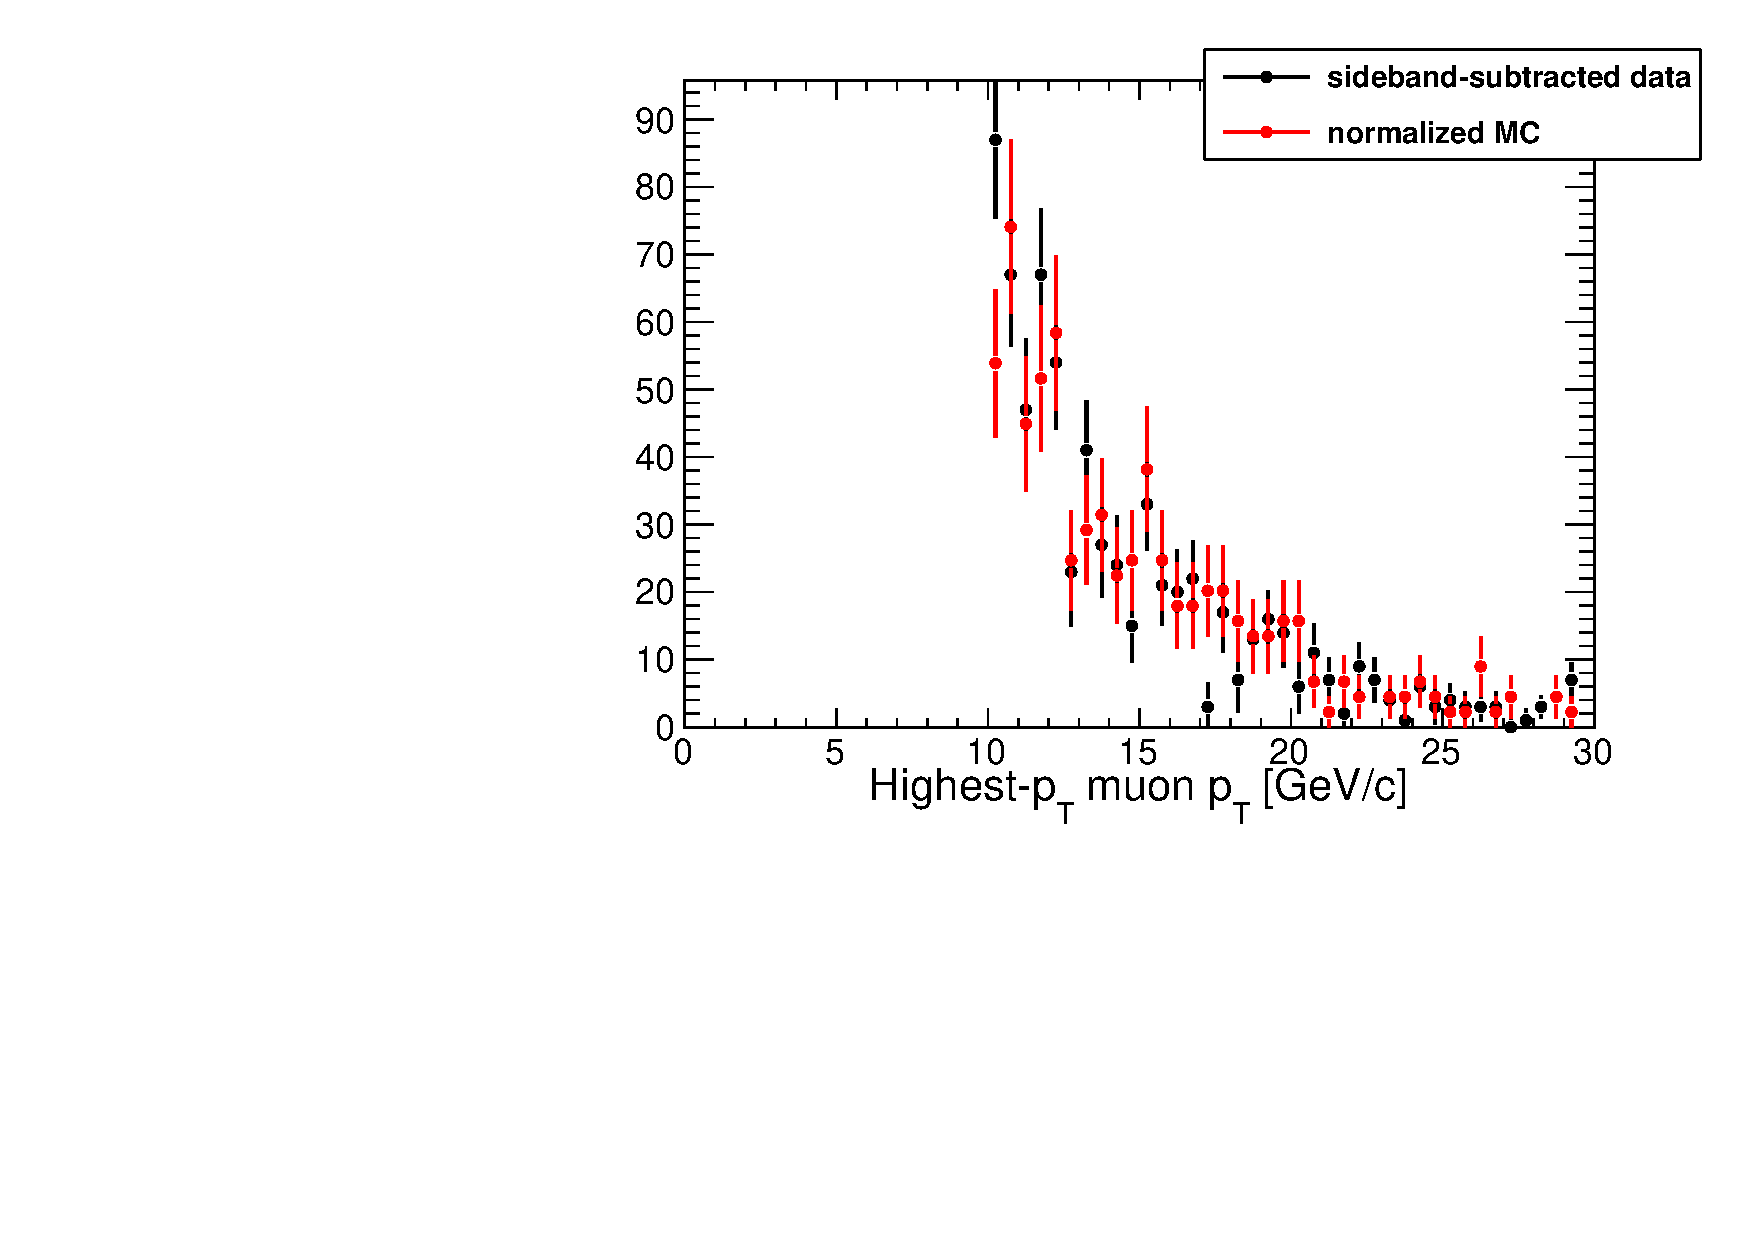
\includegraphics[width=0.5\linewidth]{phi_muon1pt.pdf}
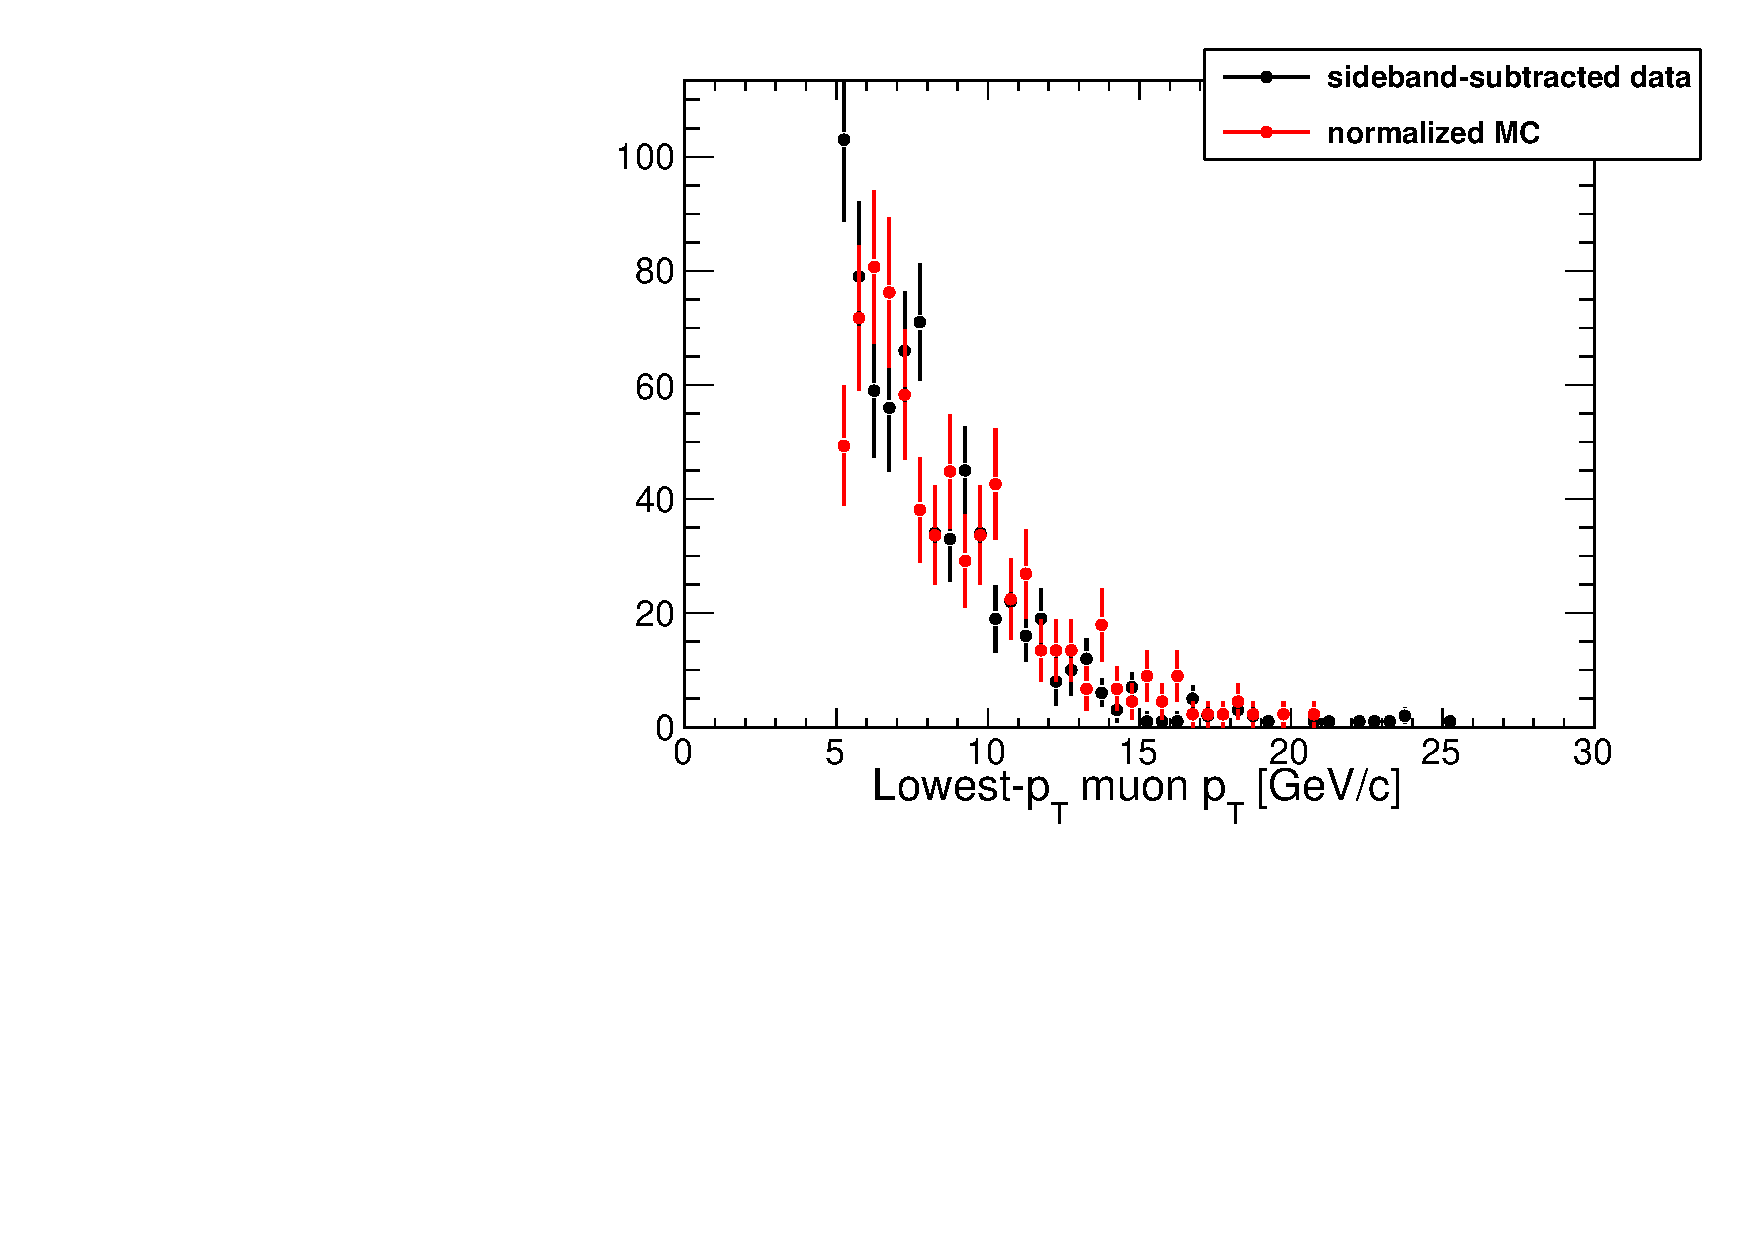
\includegraphics[width=0.5\linewidth]{phi_muon2pt.pdf}

\caption{Sideband-subtracted muon momentum distributions overlaid by
  Monte Carlo (normalized to equal number of events). \label{fig:phi_muon12pt}}
\end{figure}

\begin{figure}
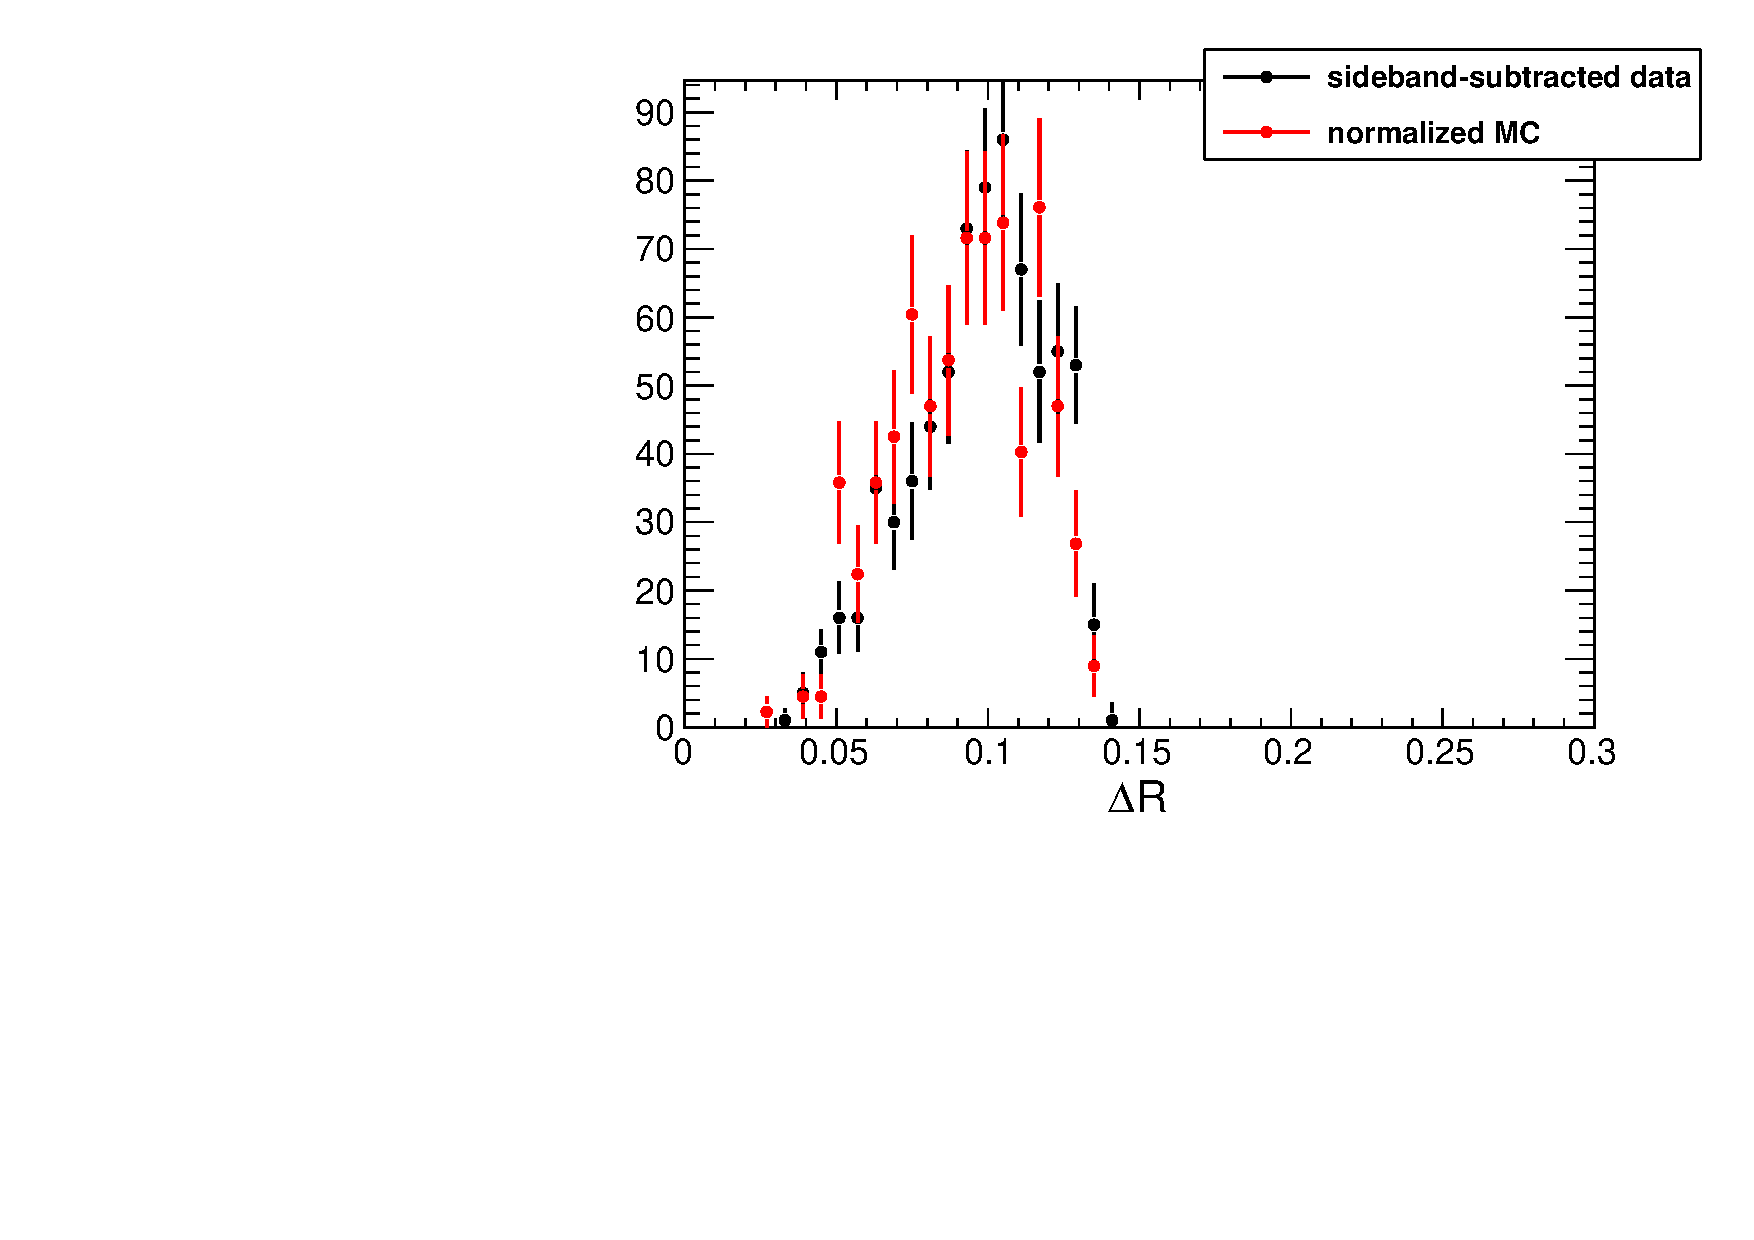
\includegraphics[width=0.5\linewidth]{phi_dr.pdf}
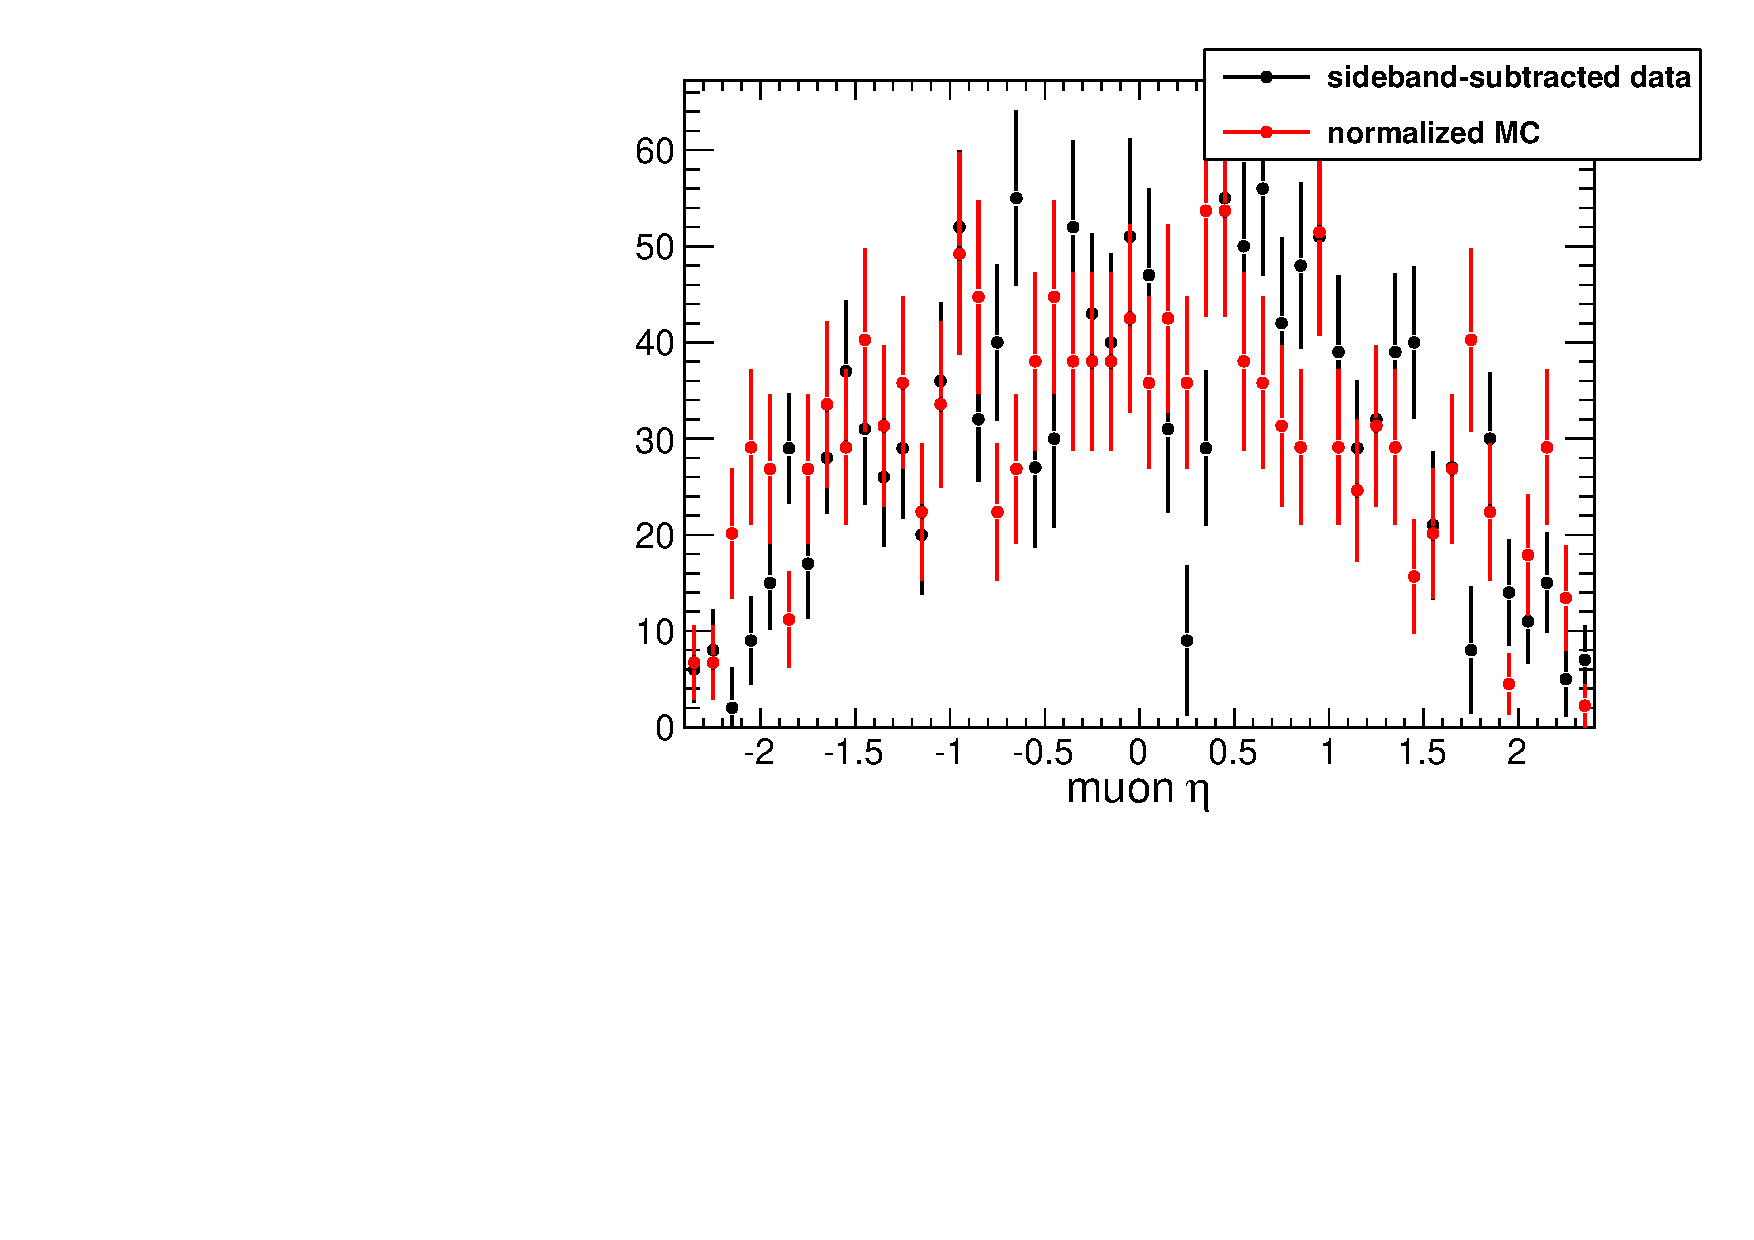
\includegraphics[width=0.5\linewidth]{phi_eta.pdf}

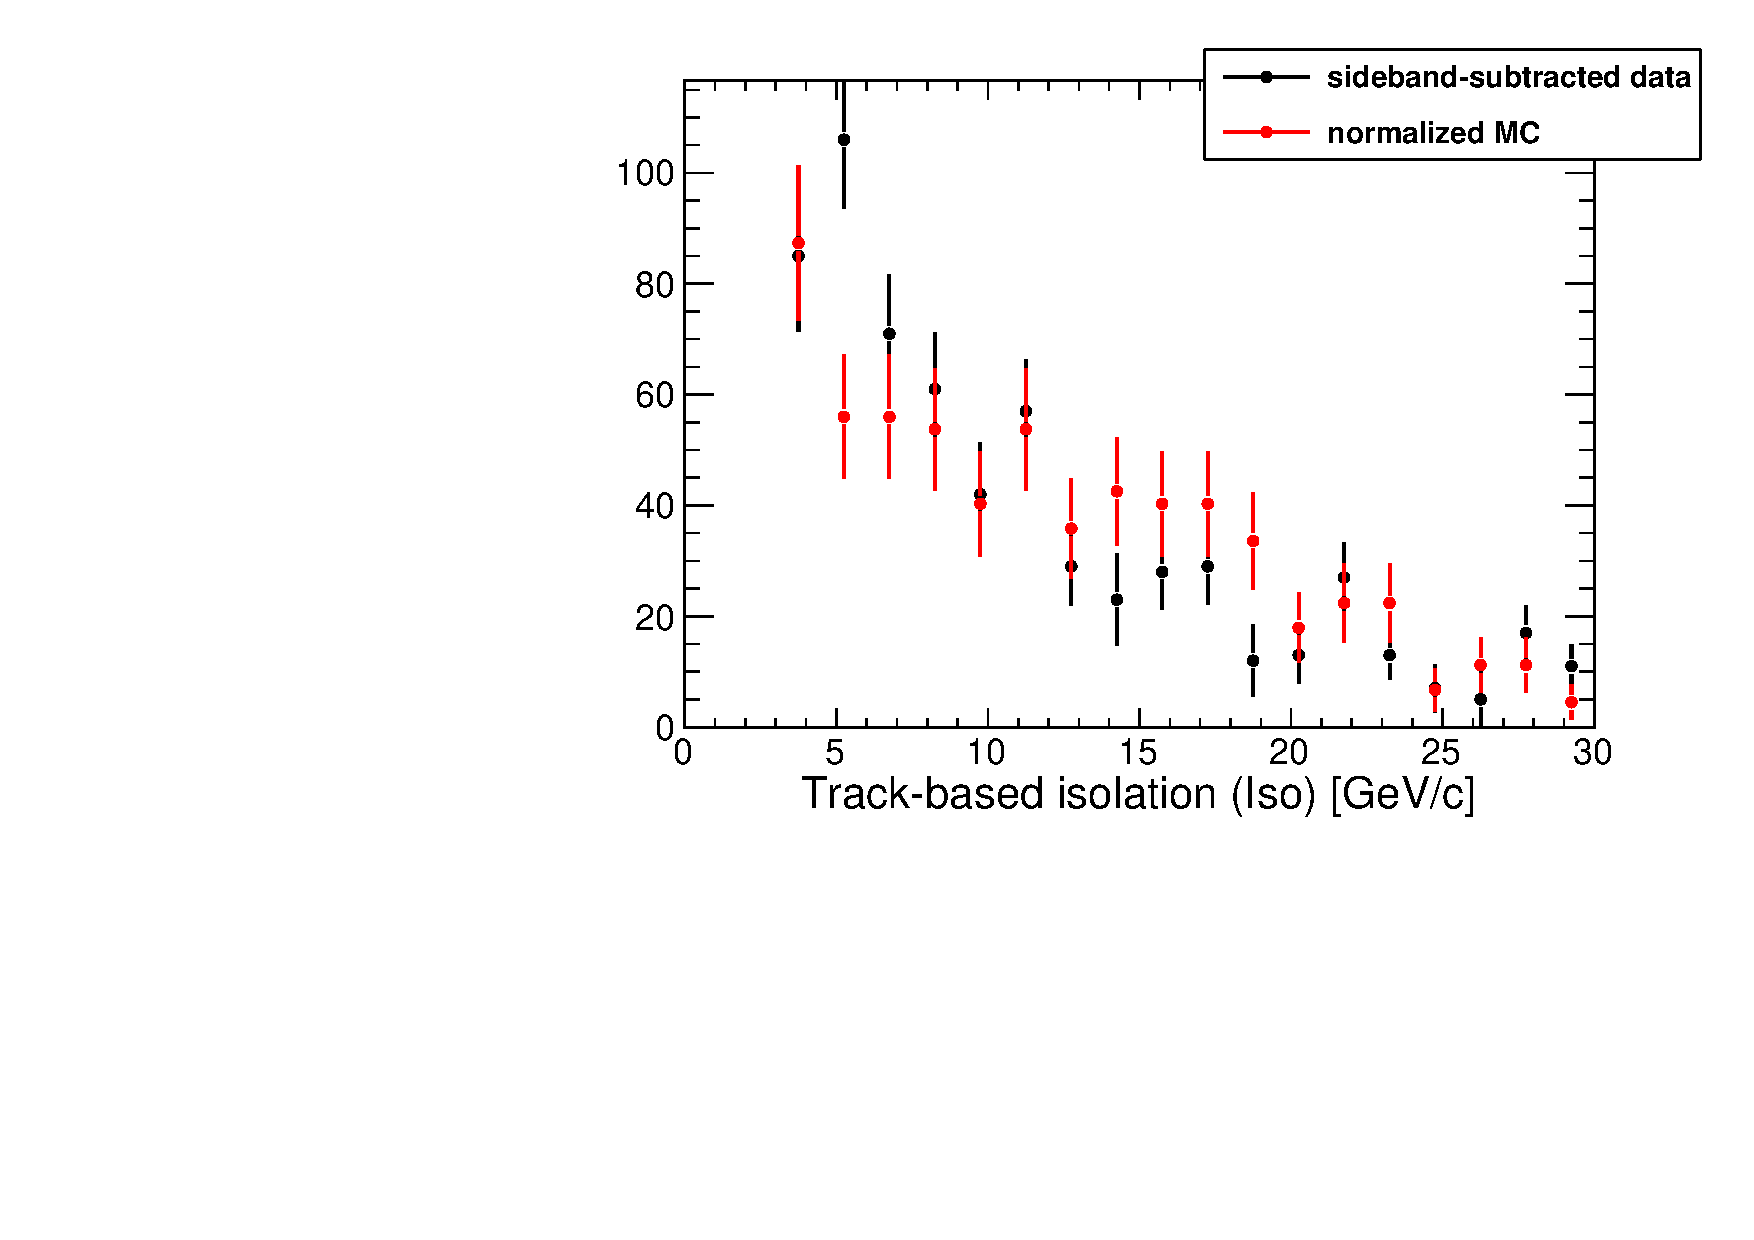
\includegraphics[width=0.5\linewidth]{phi_iso.pdf}
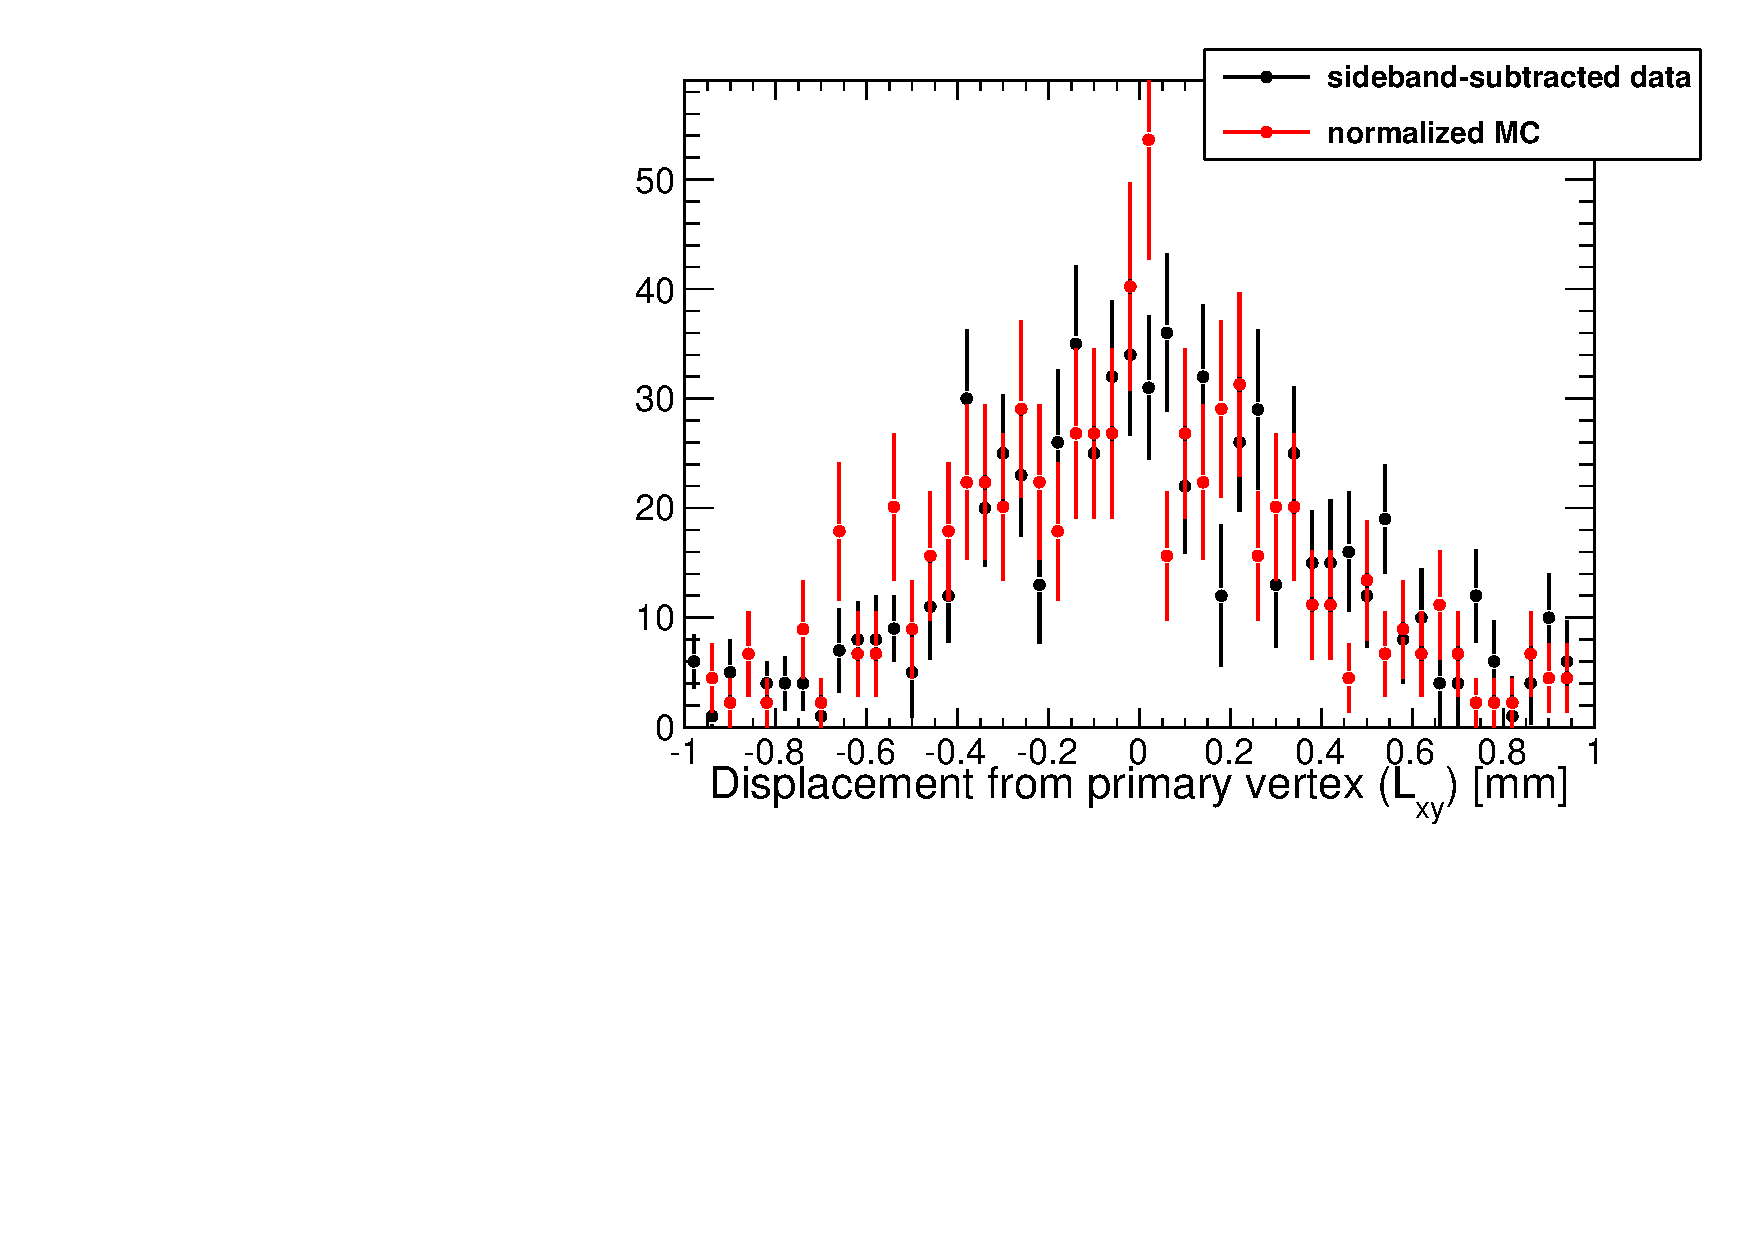
\includegraphics[width=0.5\linewidth]{phi_lxy.pdf}

\caption{Other distributions relevant for or used to define the
  $\phi(1020)$ sample. \label{fig:phi_other}}
\end{figure}

Figure~\ref{fig:phi_cuts} shows the same sideband-subtracted data
overlaid by normalized Monte Carlo for the distributions used to
define muon quality cuts: number of tracker hits, tracker
$\chi^2/N_\s{dof}$, and number of arbitrated muon segments.  All cuts
are far from the distributions except the number of segments.  The
number of segments matched to a TrackerMuon track depends on the level
of agreement between tracks propagated from the tracker and muon
segment positions and entrance angles, which are shown in
Fig.~\ref{fig:phi_residuals}.


\begin{figure}
\begin{center}
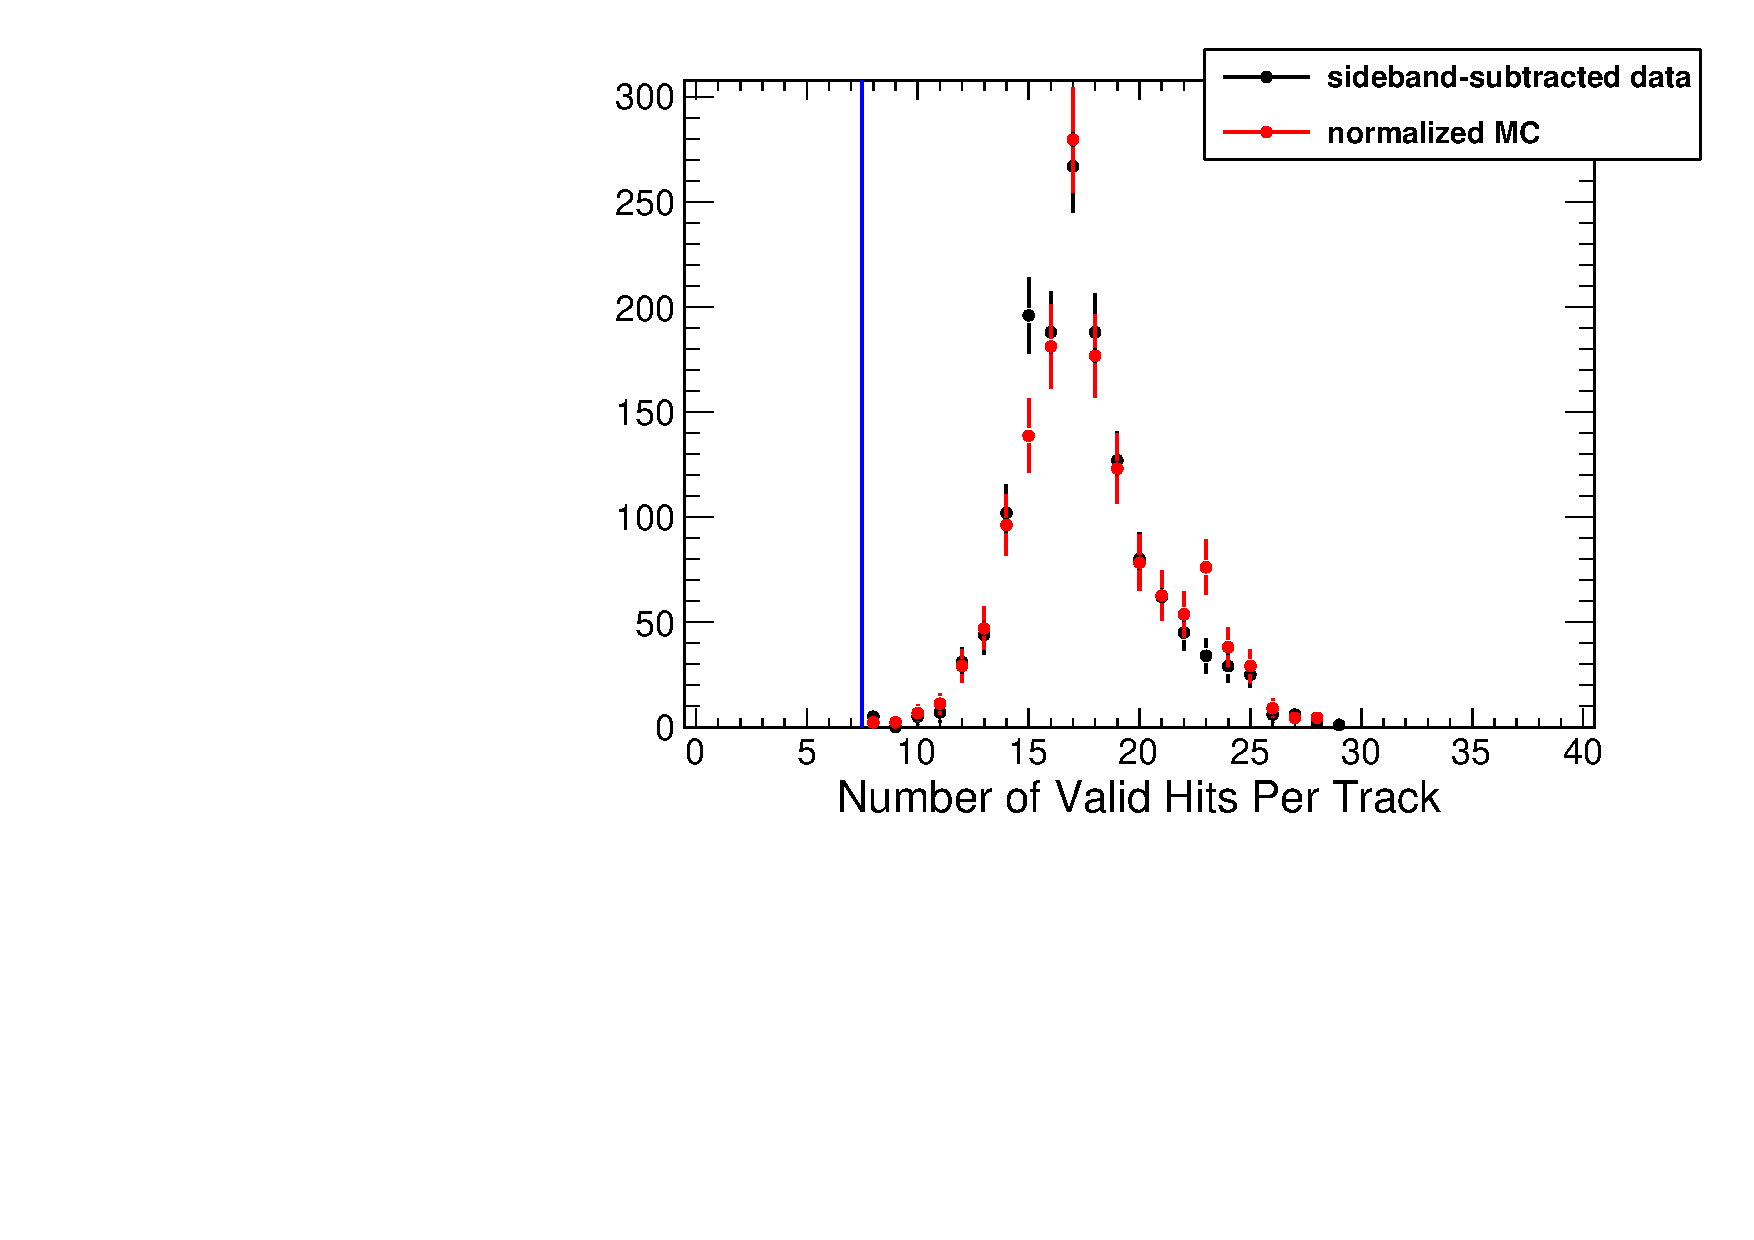
\includegraphics[width=0.48\linewidth]{phi_hits.pdf}
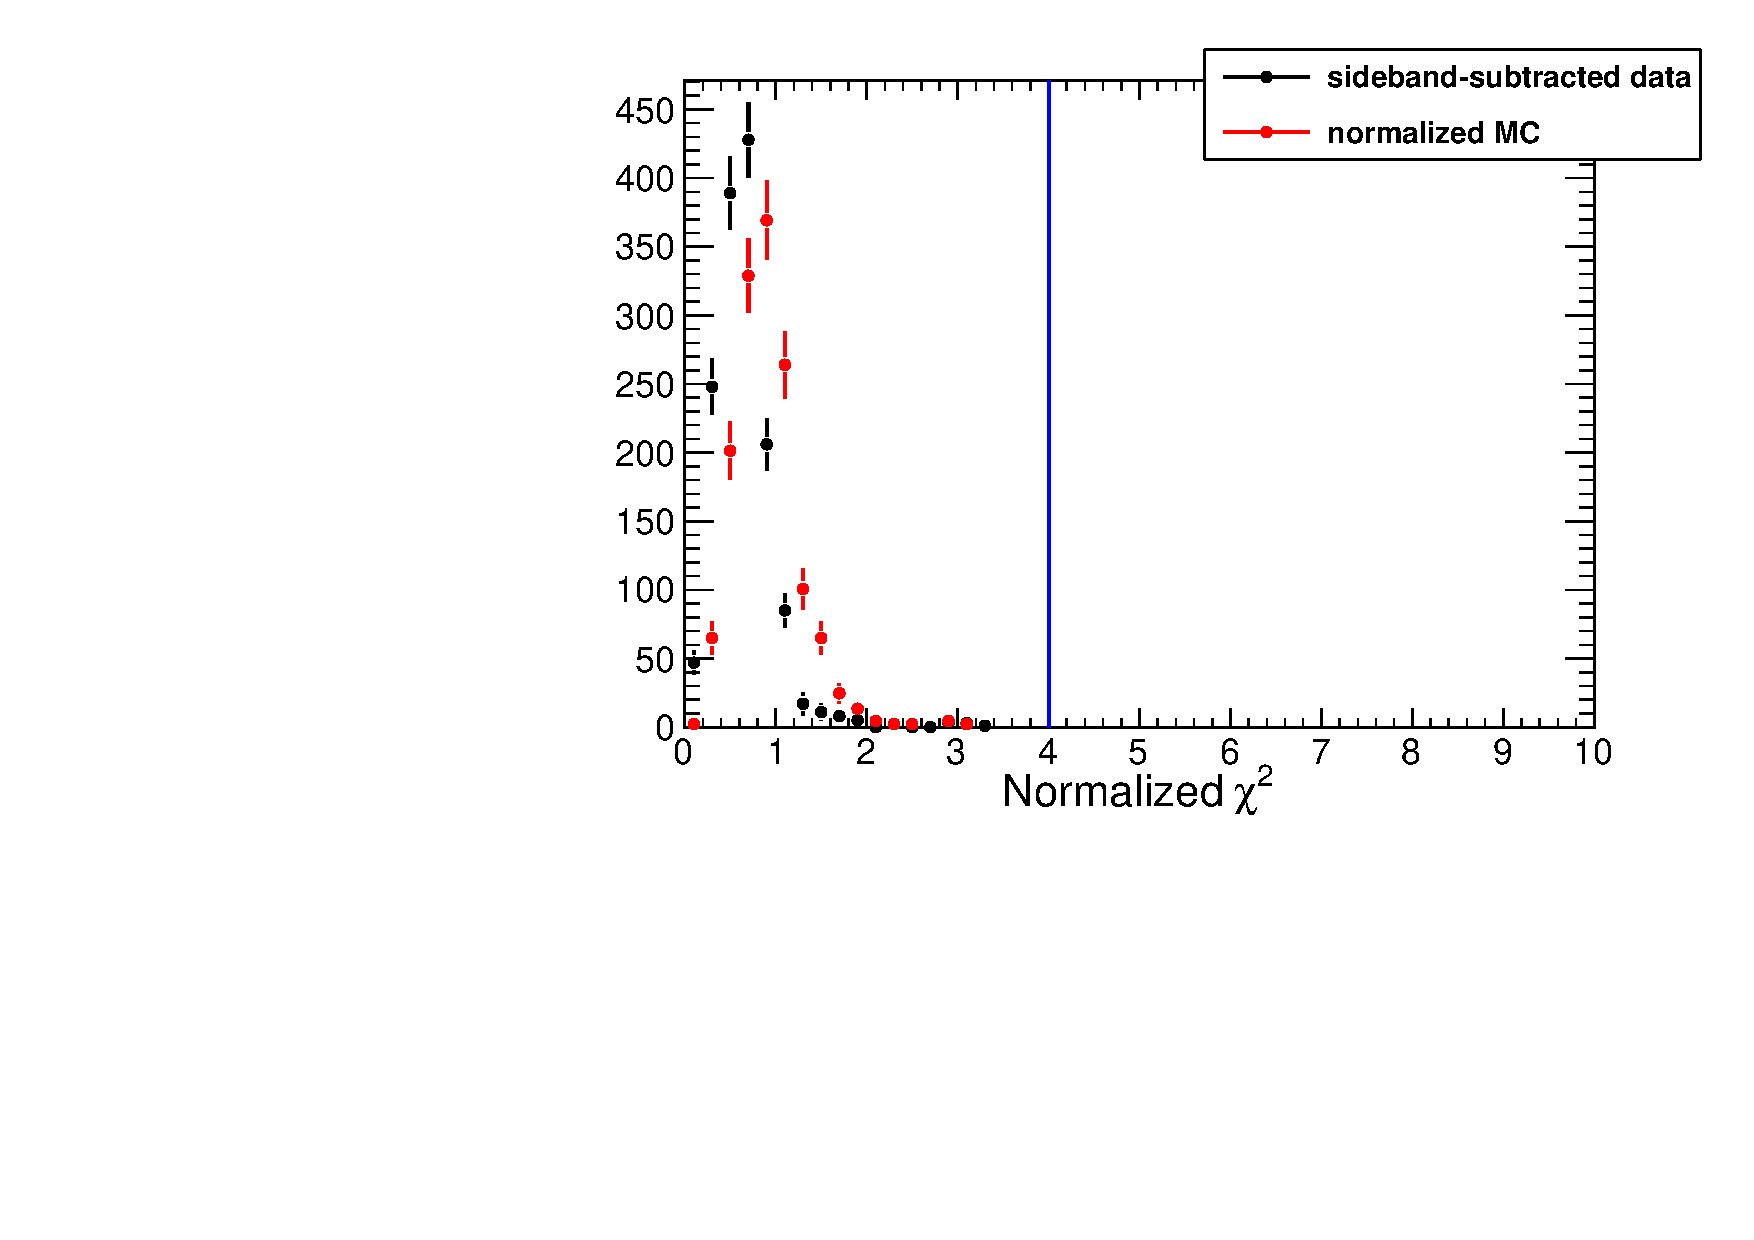
\includegraphics[width=0.48\linewidth]{phi_normchi2.pdf}

\vspace{0.25 cm}
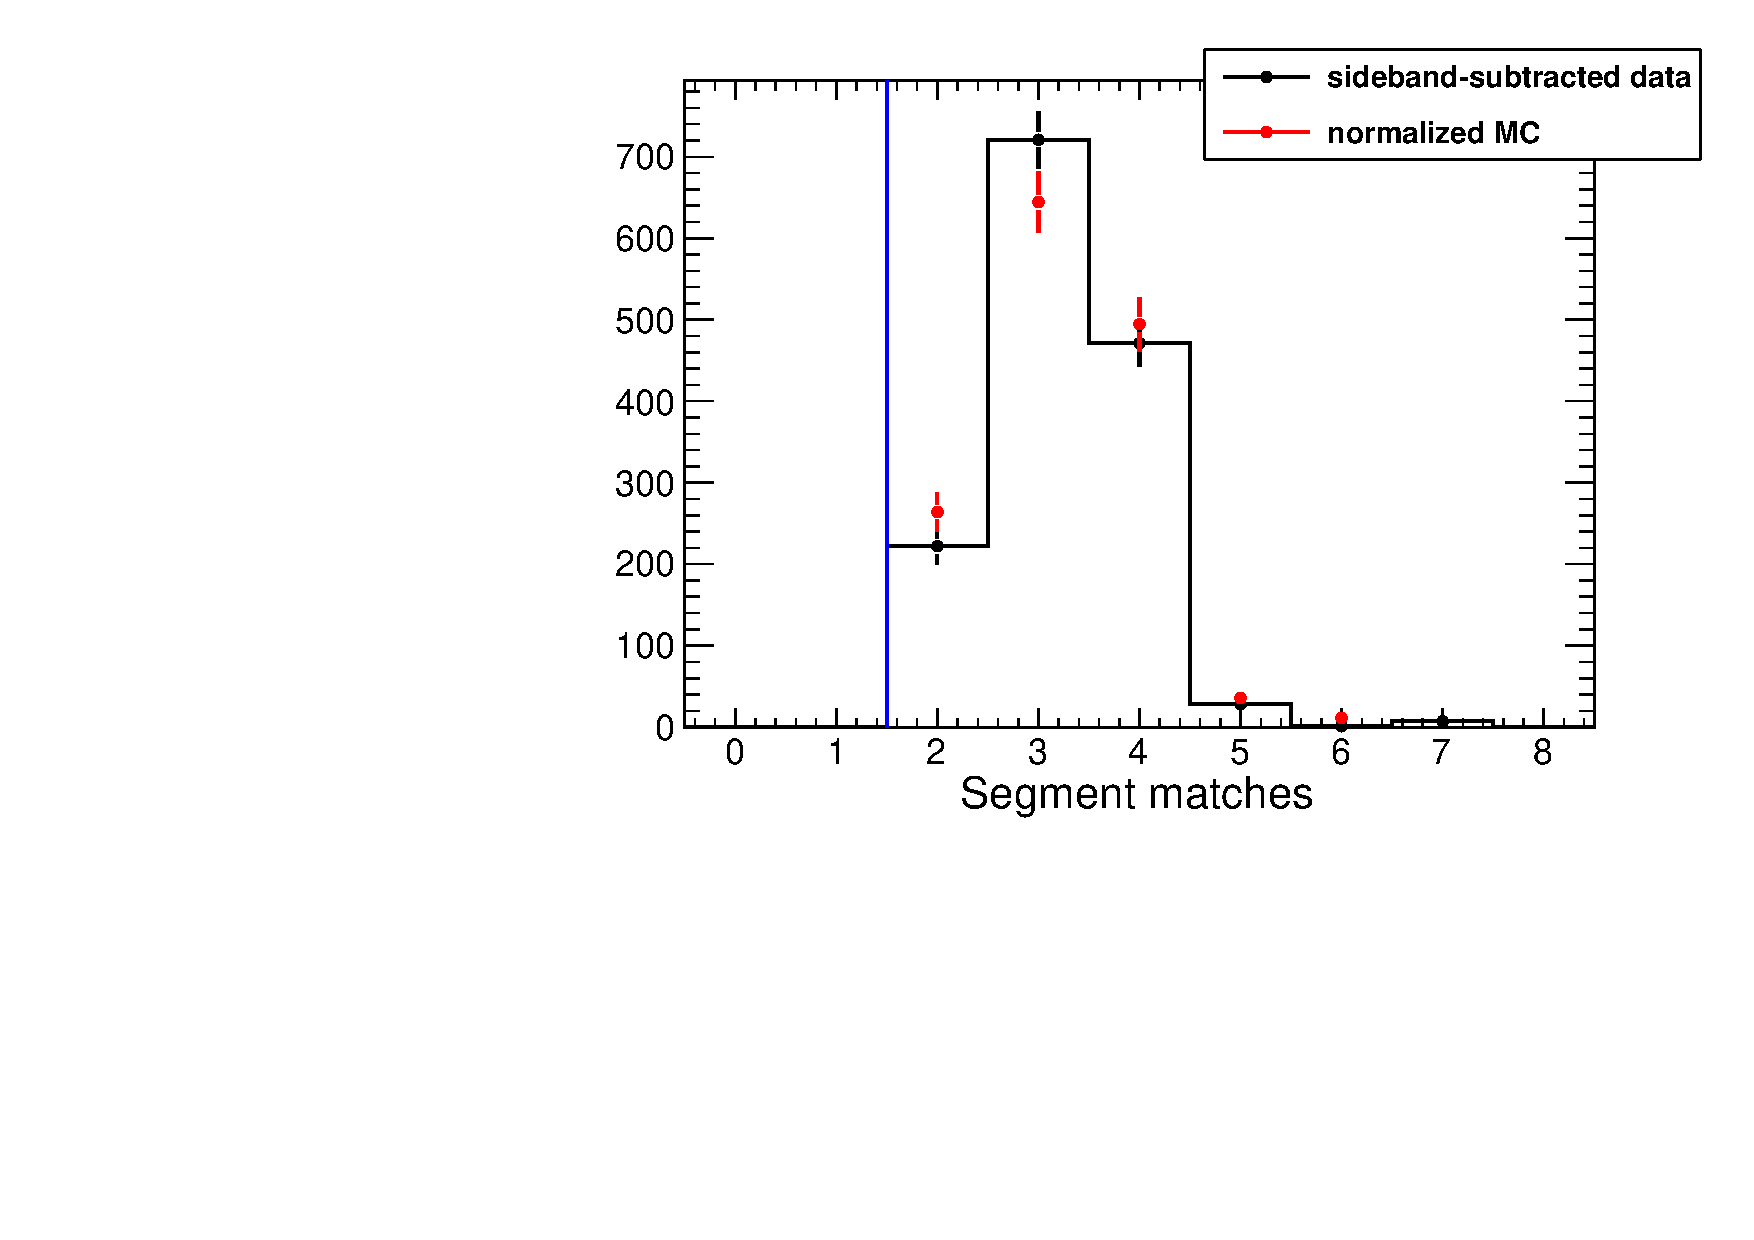
\includegraphics[width=0.48\linewidth]{phi_matches.pdf}
\end{center}

\caption{Distributions of track quality cuts (top row) and muon
  quality cuts (bottom) with cut thresholds indicated in blue.  All
  cuts have been applied in all distributions. \label{fig:phi_cuts}}
\end{figure}

\begin{figure}
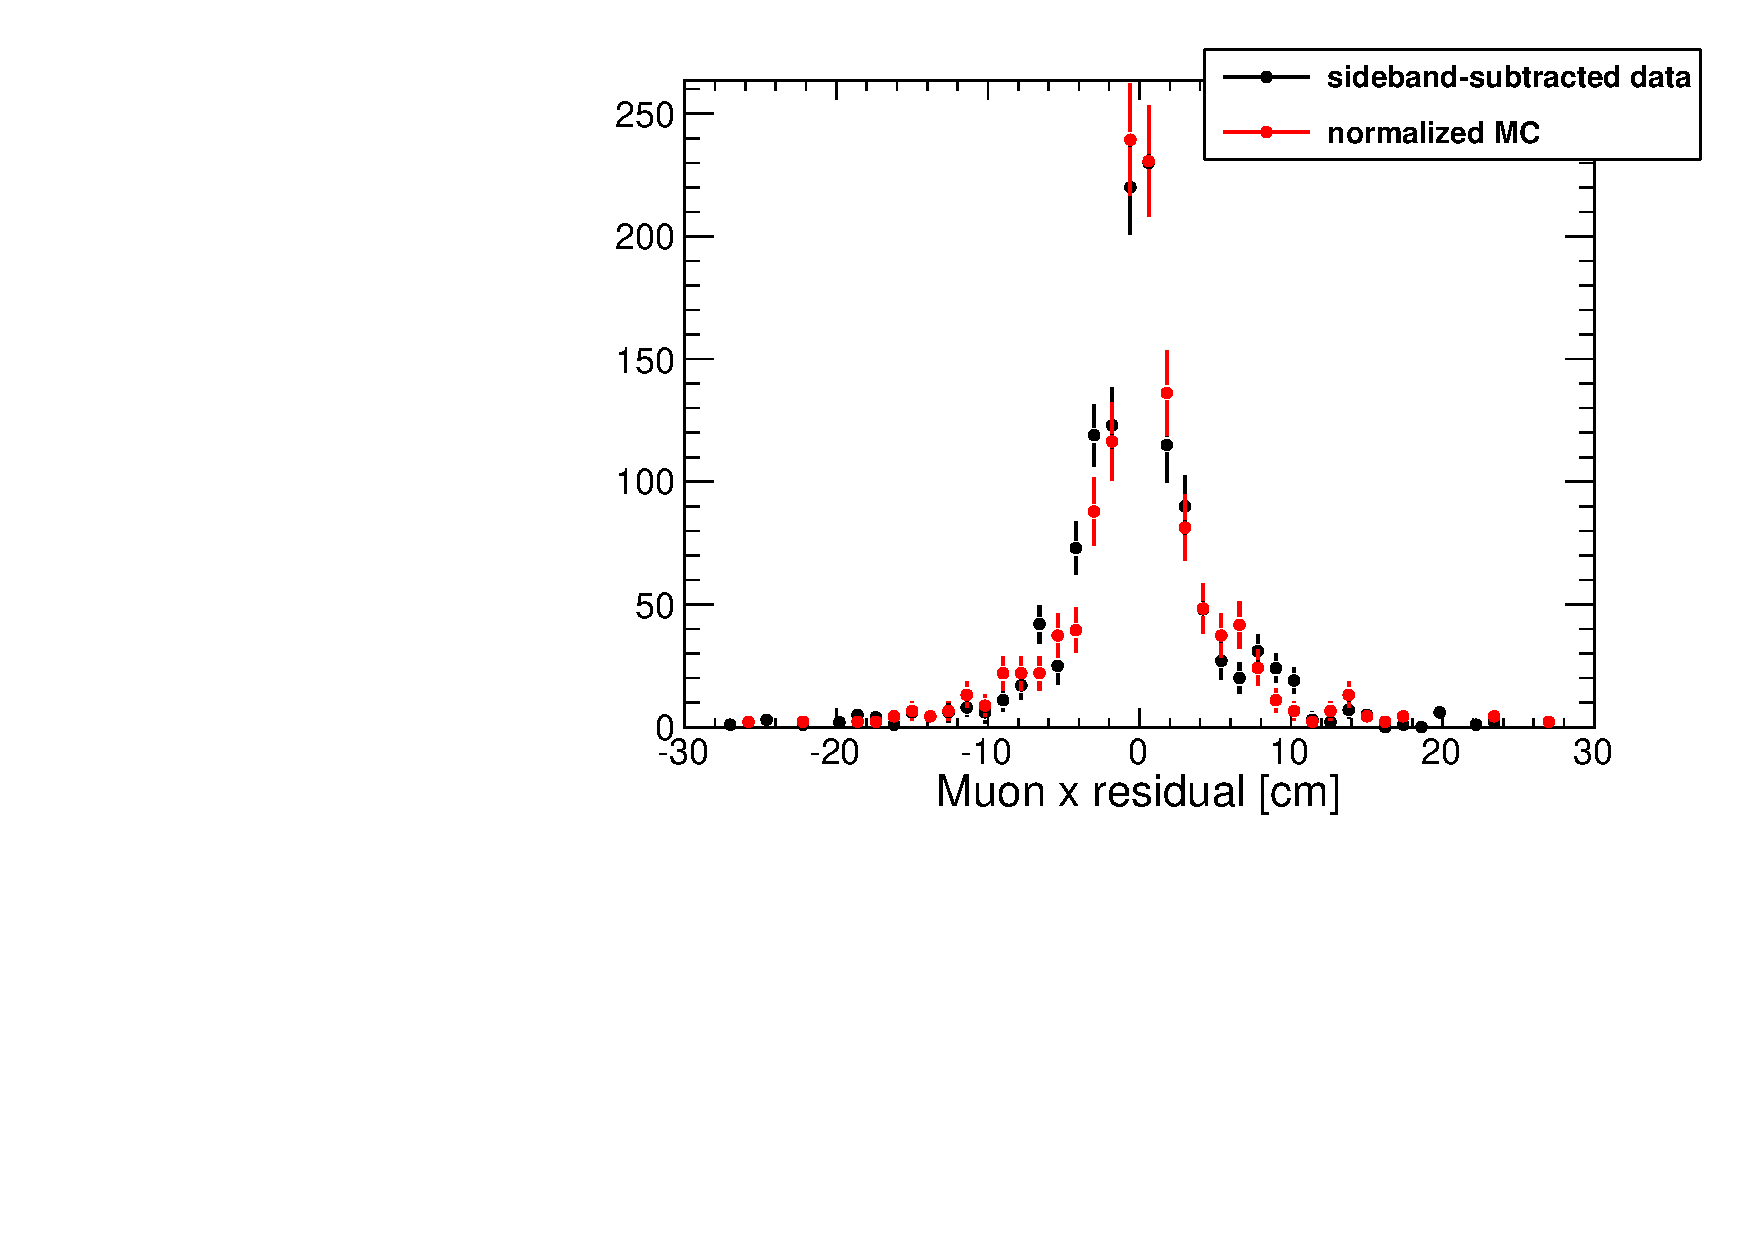
\includegraphics[width=0.5\linewidth]{phi_st1x.pdf}
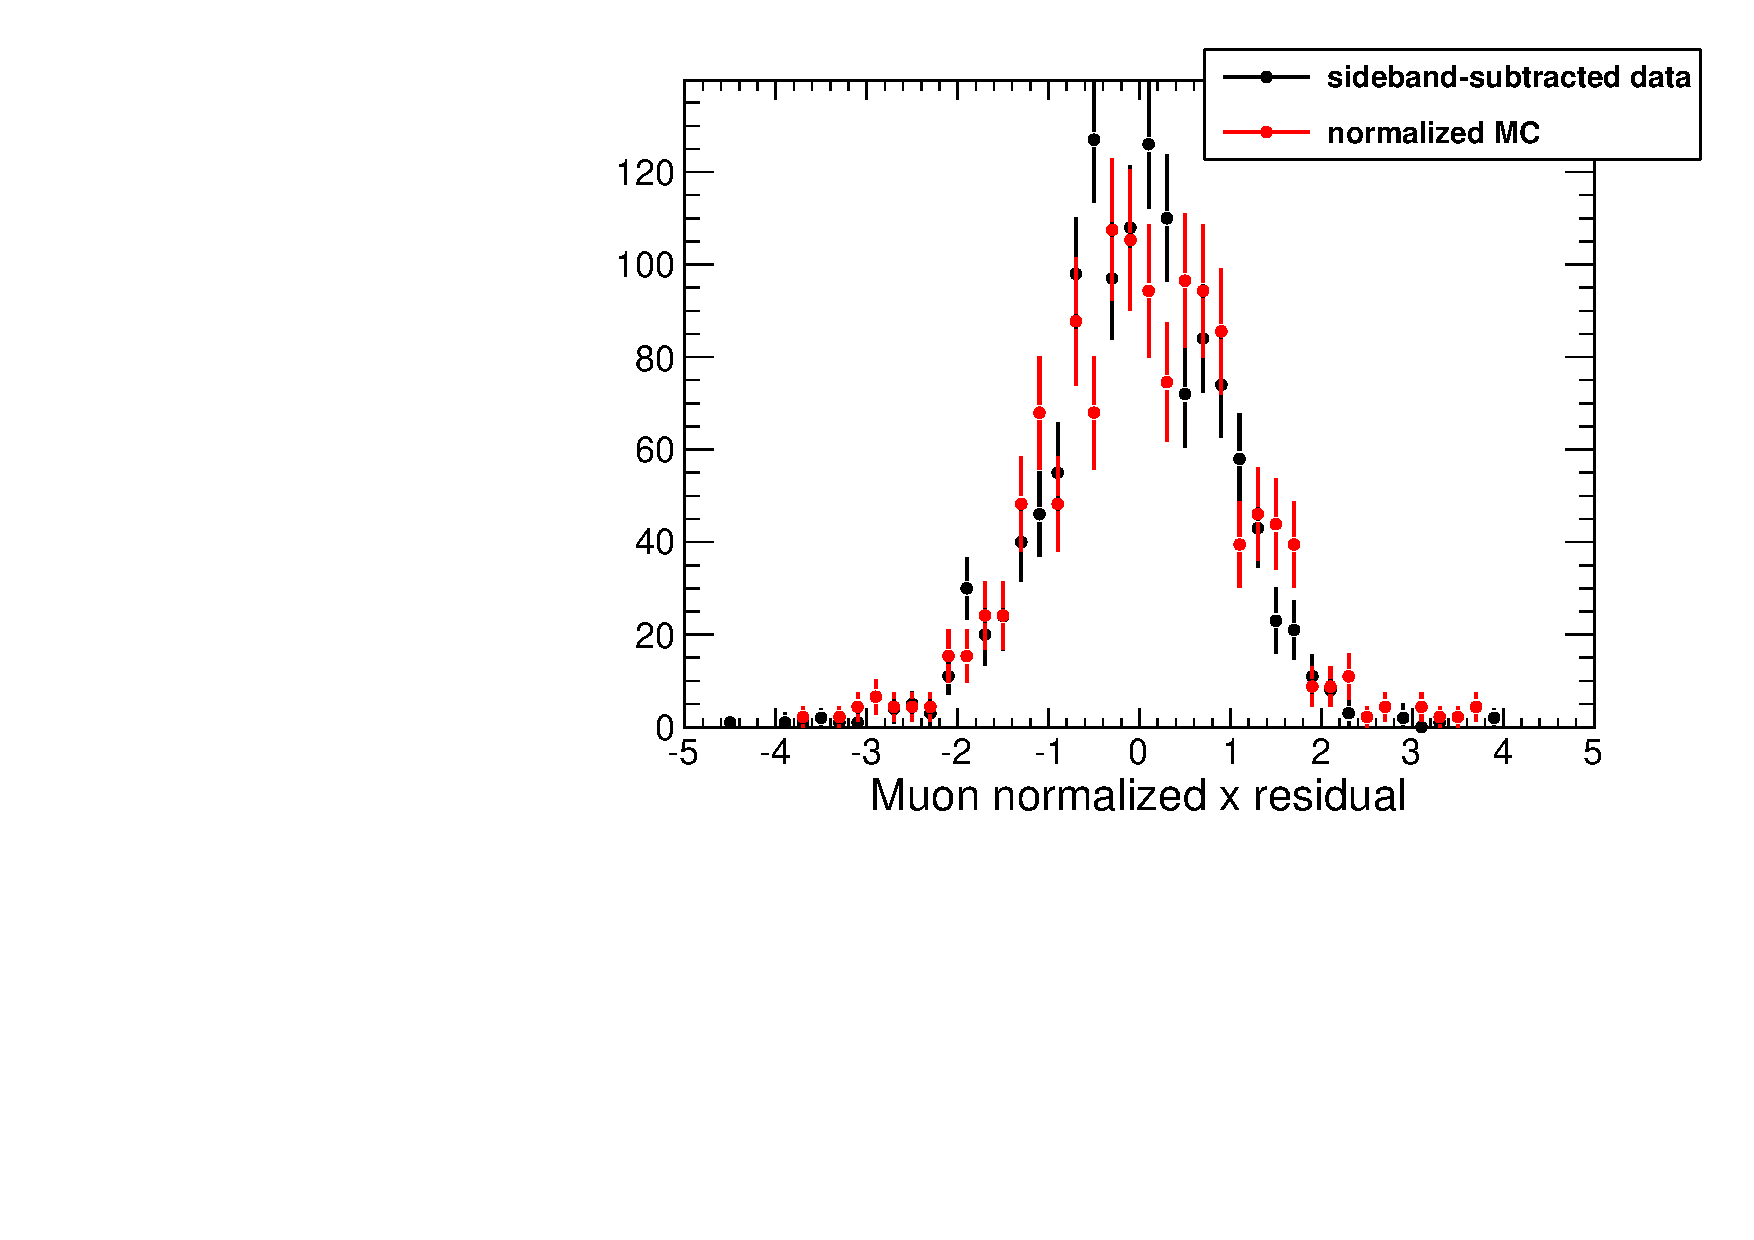
\includegraphics[width=0.5\linewidth]{phi_st1xsig.pdf}

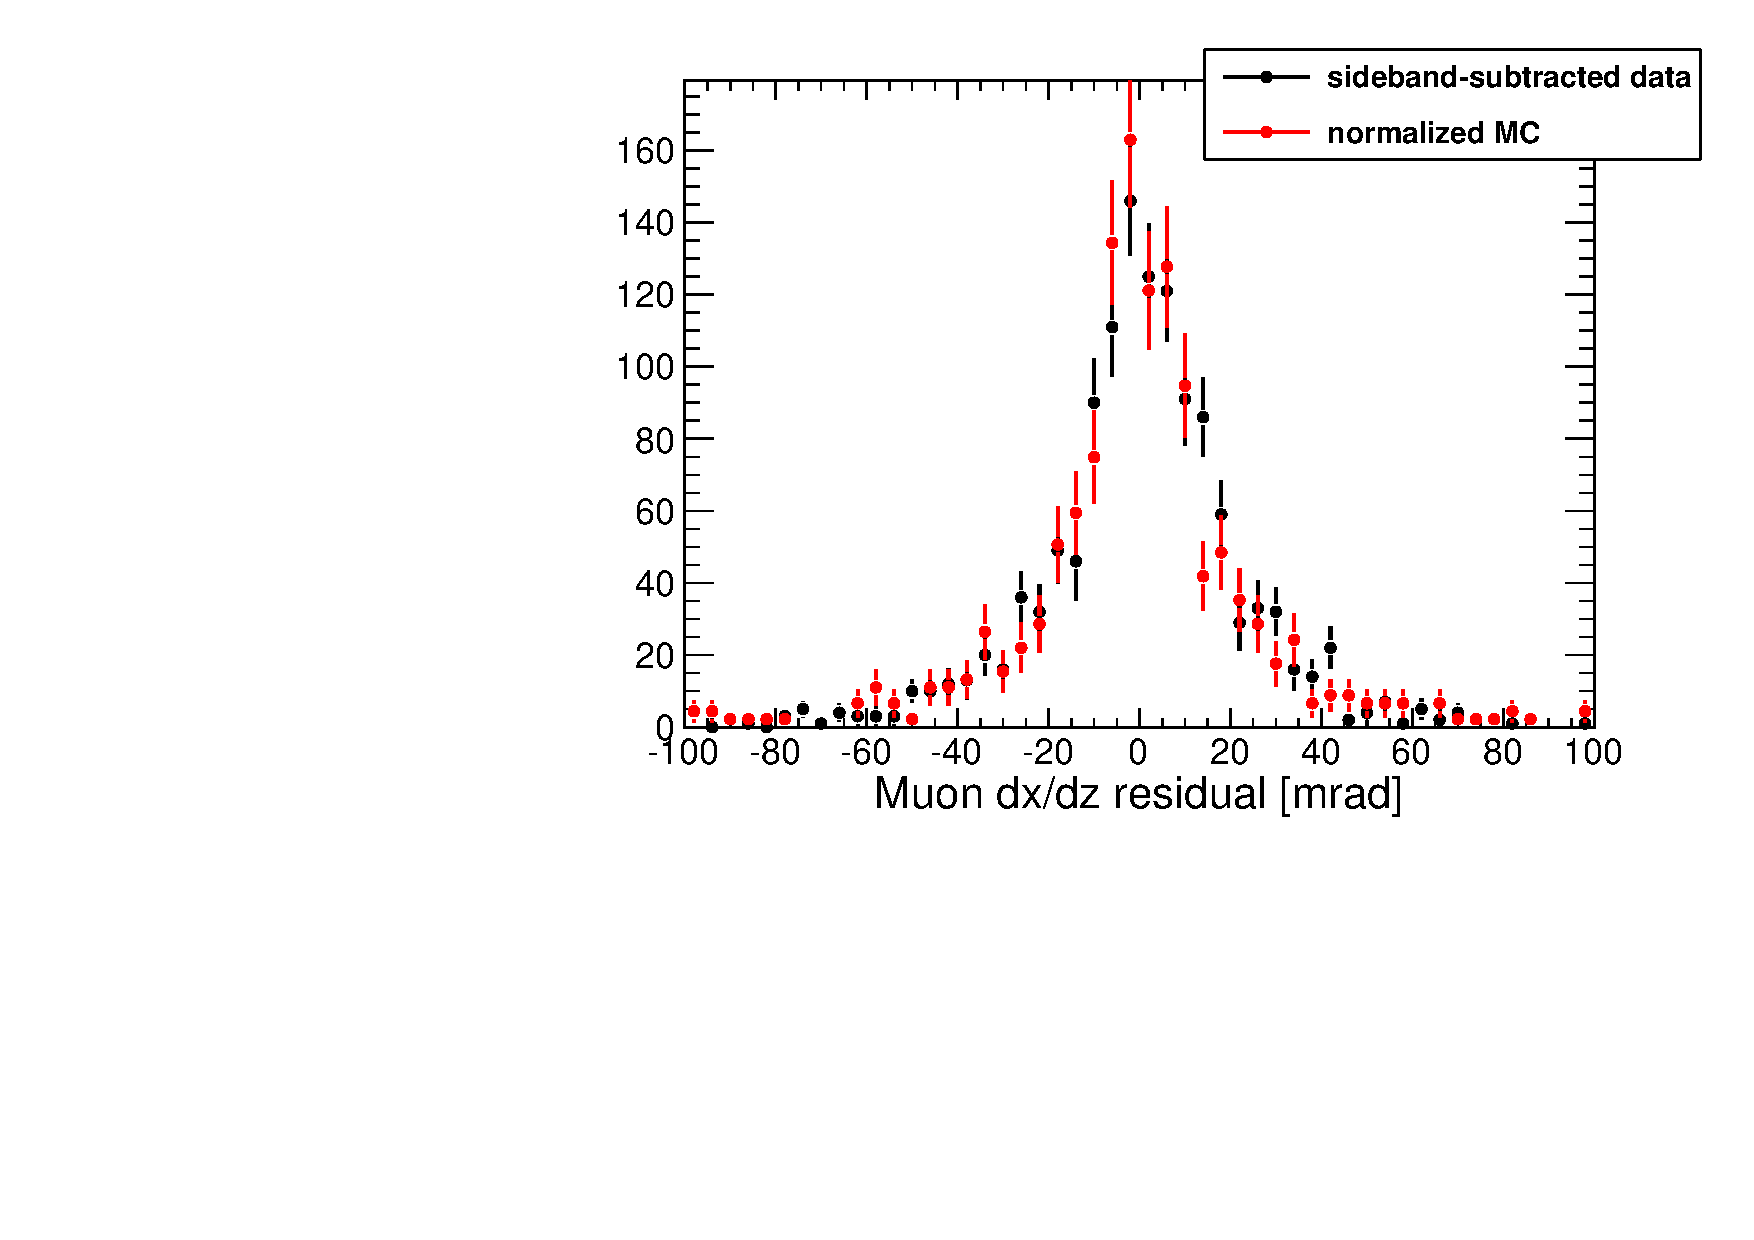
\includegraphics[width=0.5\linewidth]{phi_st1dxdz.pdf}
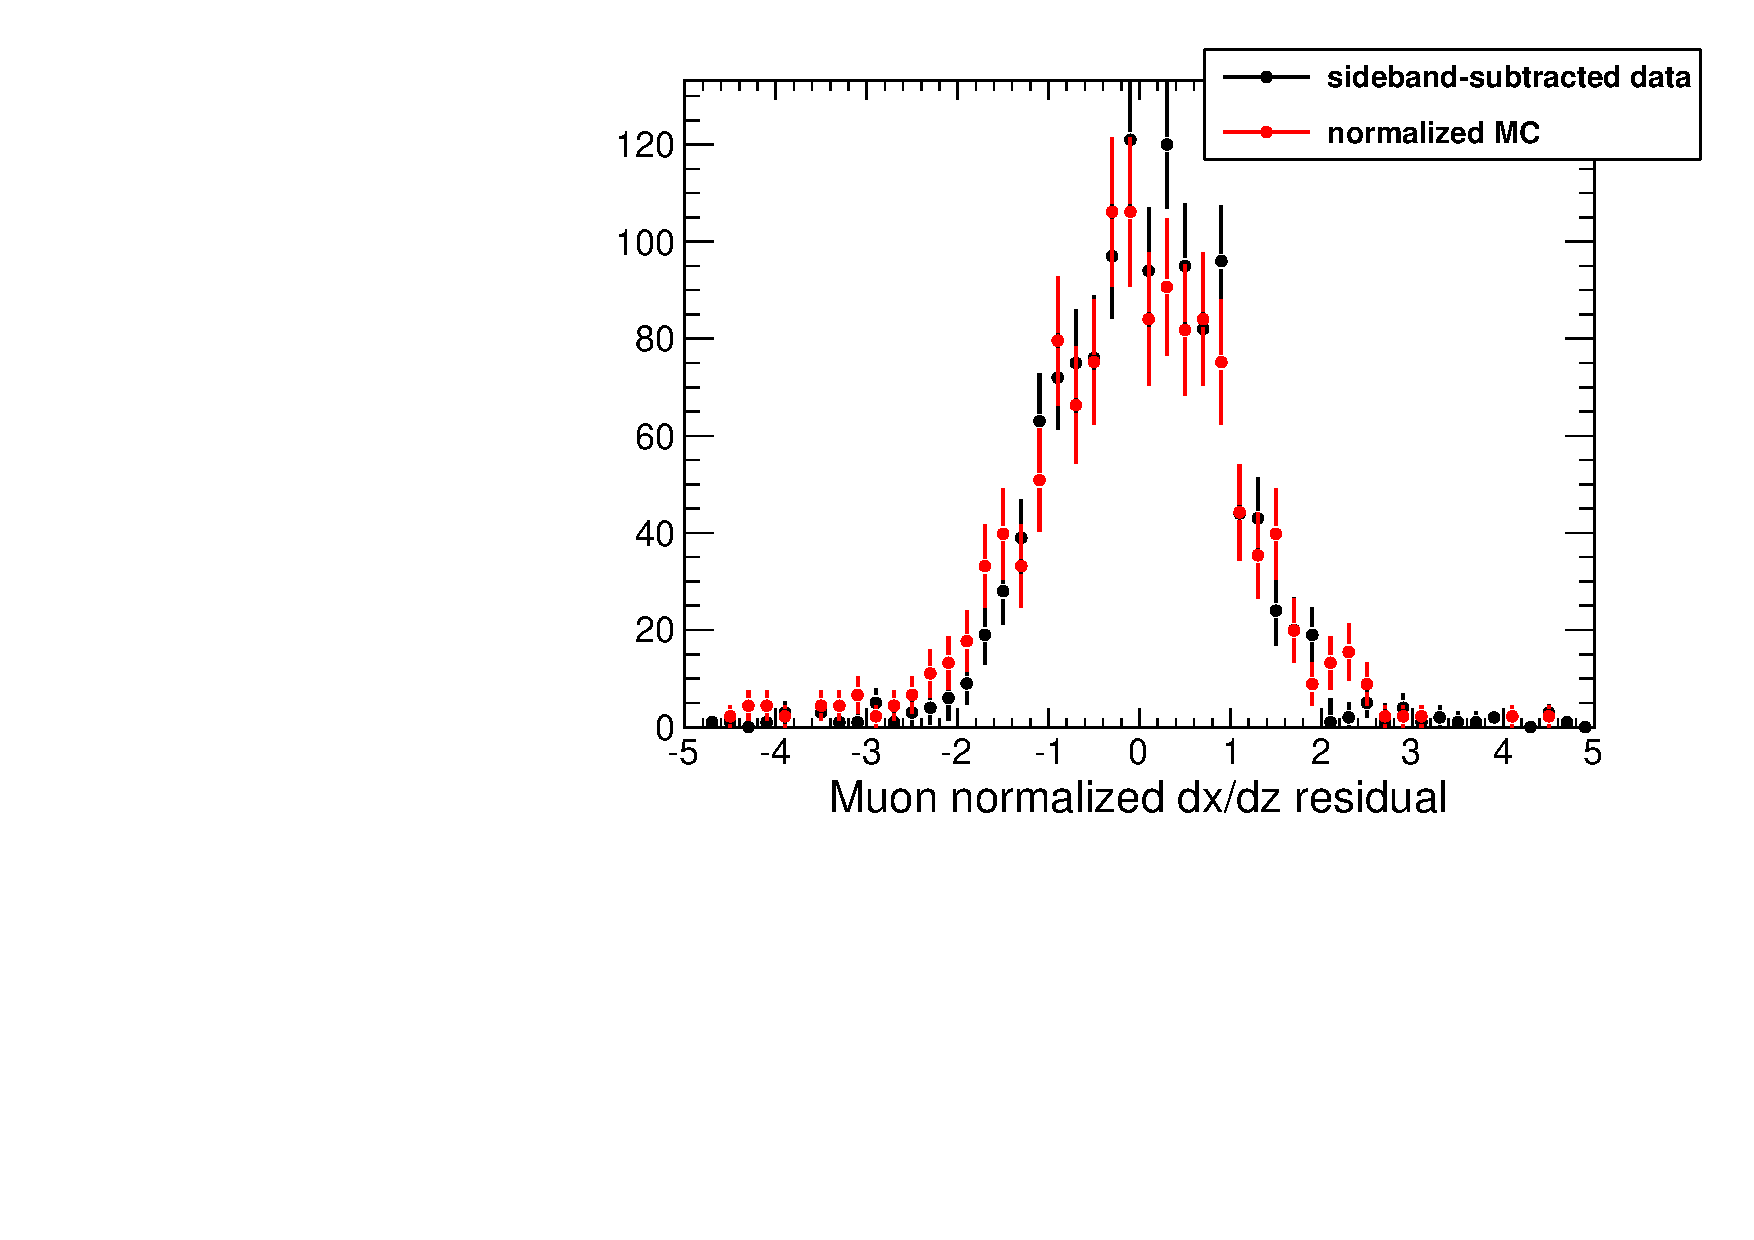
\includegraphics[width=0.5\linewidth]{phi_st1dxdzsig.pdf}

\caption{Distance between propagated track and muon segment in the
  magnetic field bending plane ($x$, top-left), the same normalized by
  uncertainty (top-right), the difference in entrance angle ($dx/dz$,
  bottom-left), and the same normalized by uncertainty (bottom-right).
  These are relevant for determining the number of muon segments
  matched to a TrackerMuon. \label{fig:phi_residuals}}
\end{figure}

The Monte Carlo sample used in this study and all signal samples used
in the main analysis were produced using ideal alignment and
calibration conditions.  The data in this $\phi(1020)$ study is a
combination of Sep17ReReco (2010A) and PromptReco (2010B), unlike the
main analysis, which uses Dec22ReReco.  The only observed discrepancy
between data and Monte Carlo is in the $\chi^2/N_\s{dof}$ distribution
(Fig.~\ref{fig:phi_cuts} top-right), in which the Monte Carlo peaks at
one but the data peaks lower than one.  This {\it could} be because
the tracker alignment uses artificially inflated Alignment Position
Errors (APEs) in PromptReco for safety (this was the case in early LHC
running\ldots\ not sure if it's still true\ldots\ {\bf FIXME}).  The
muon residuals distributions (Fig.~\ref{fig:phi_residuals}) are
completely insensitive to muon alignment conditions for
$\sim$20~GeV/$c$ muon momenta because of the dominance of multiple
scattering in the propagation.

\section{Conclusions}

Muon segment assignment for muons whose trajectories cross in the muon
system is the dominant efficiency systematic for a wide range of
opening angles.  However, efficiency losses in the tracker could play
a significant role for 150--300~GeV/$c$ muons.  An 8\% loss in
efficiency is observed in pair-gun MC for $\Delta R < 0.01$ muon
pairs, though such a high boost is a special case in our analysis.
The simulation was tested for moderately low opening angles ($0.05 <
\Delta R < 0.15$) using the $\phi(1020)$ resonance, though the region
where the tracker begins to be inefficient for nearby muons is
orthogonal to this or any test using Standard Model resonances.

\end{document}
